\documentclass{article}[12pt, a4paper]
\topmargin = 15pt

\usepackage{graphics}
\usepackage[top=1in, bottom=1.25in, left=36mm, right=36mm]{geometry}
\usepackage[hidelinks]{hyperref}
\usepackage[utf8]{inputenc}
\usepackage{parskip}
\usepackage{silence}
\usepackage{multirow}
\WarningFilter{latex}{Text page 2 contains only floats}
 
%\VignetteIndexEntry{Downscaling}
%\vignetteDepends{downscale}

\graphicspath{{figures/}}

\graphicspath{{figures/}}






\usepackage{Sweave}
\begin{document}
\Sconcordance{concordance:Downscaling.tex:Downscaling.Rnw:%
1 22 1 1 6 1 1 1 0 998 1}

\Sconcordance{concordance:Downscaling.tex:Downscaling.Rnw:%
1 22 1 1 6 1 1 1 0 998 1}


\title{Downscaling species occupancy: \\ an introduction and tutorial}
\author{Charles J. Marsh}
\date{\today}
\maketitle
\tableofcontents

\newpage
\section{Introduction to downscaling}

In order to assess and manage the status of a species we need to know the abundance of individuals in the population(s) and their changes over time. For the vast majority of species this information is unobtainable, however one important proxy of true abundance and extinction risk is the area occupied by the species. For example, the area of occupancy (AOO) is a little-used measure of conservation status in the IUCN red list (IUCN 2014). Although easier to estimate than true abundance, the difficulty in estimating AOO lies in the extensive sampling required across the full range of the species at a grain size sufficiently fine to give meaningful estimates (and this grain size may vary with taxon, habitat or region). For the majority of species this is still impractical or unfeasible at these grain sizes. However, as we estimate occupancy at increasing grain sizes we increase our confidence in our presence-absence predictions. Such coarse-grain atlas data, generally generated from opportunistic recording over extended periods of time, are much more widely available. However, at such coarse grain sizes we also lose resolution in our status estimates as occupancy rates at large grain sizes are less closely correlated with true abundance (Hartley and Kunin 2003).

A solution is to employ the occupancy-area relationship (OAR); the increase in the  area occupied by a species as grain size increases (Kunin 1998). If the relationship can be described at these coarser grain sizes where confidence is high, then we can extrapolate to predict occupancy at the fine grain sizes necessary for conservation assessments that are more closely related to the true abundance, distribution and conservation status.

Many models have been proposed to describe this geometric relationship, and it appears that no one model consistently provides the best predictions (Azaele et al. 2012, Barwell et al. 2014). This package provides functions for ten commonly applied models, along with functions for preparing coarse-scale data, plotting results, and an ensemble method for running multiple models and averaging their predictions.

\newpage
\section{Using the downscale package}

The general flow of the \texttt{downscale} package is presented in fig. \ref{fig:Flow}. The package is based around seven user functions:  \texttt{upgrain.threshold}, \texttt{upgrain}, \texttt{downscale}, \texttt{predict}, \texttt{hui.downscale}, \texttt{plot}, and \texttt{ensemble.downscale}. Ten downscaling models are available (Nachman, power law, logistic, poisson, negative binomial, generalised negative binomial, improved negative binomial, finite negative binomial, Thomas and Hui models). Details of all models can be found in the help files, and in the supplementary information of Barwell et al. 2014. 

The user may input three types of data:
\begin{enumerate} \itemsep1pt \parskip0pt 
\item [1)] A data frame of grain sizes (cell area) and occupancies in that order;
\item [2)] A data frame of cell coordinates and presence-absence data (presence = 1; absence = 0). Column names must be “lon”, “lat”, and “presence” in that order;
\item [3)] A raster layer of presence-absence data (presence = 1; absence = 0; no data = NA).
\end{enumerate}

\begin{figure}[!ht]
\centering
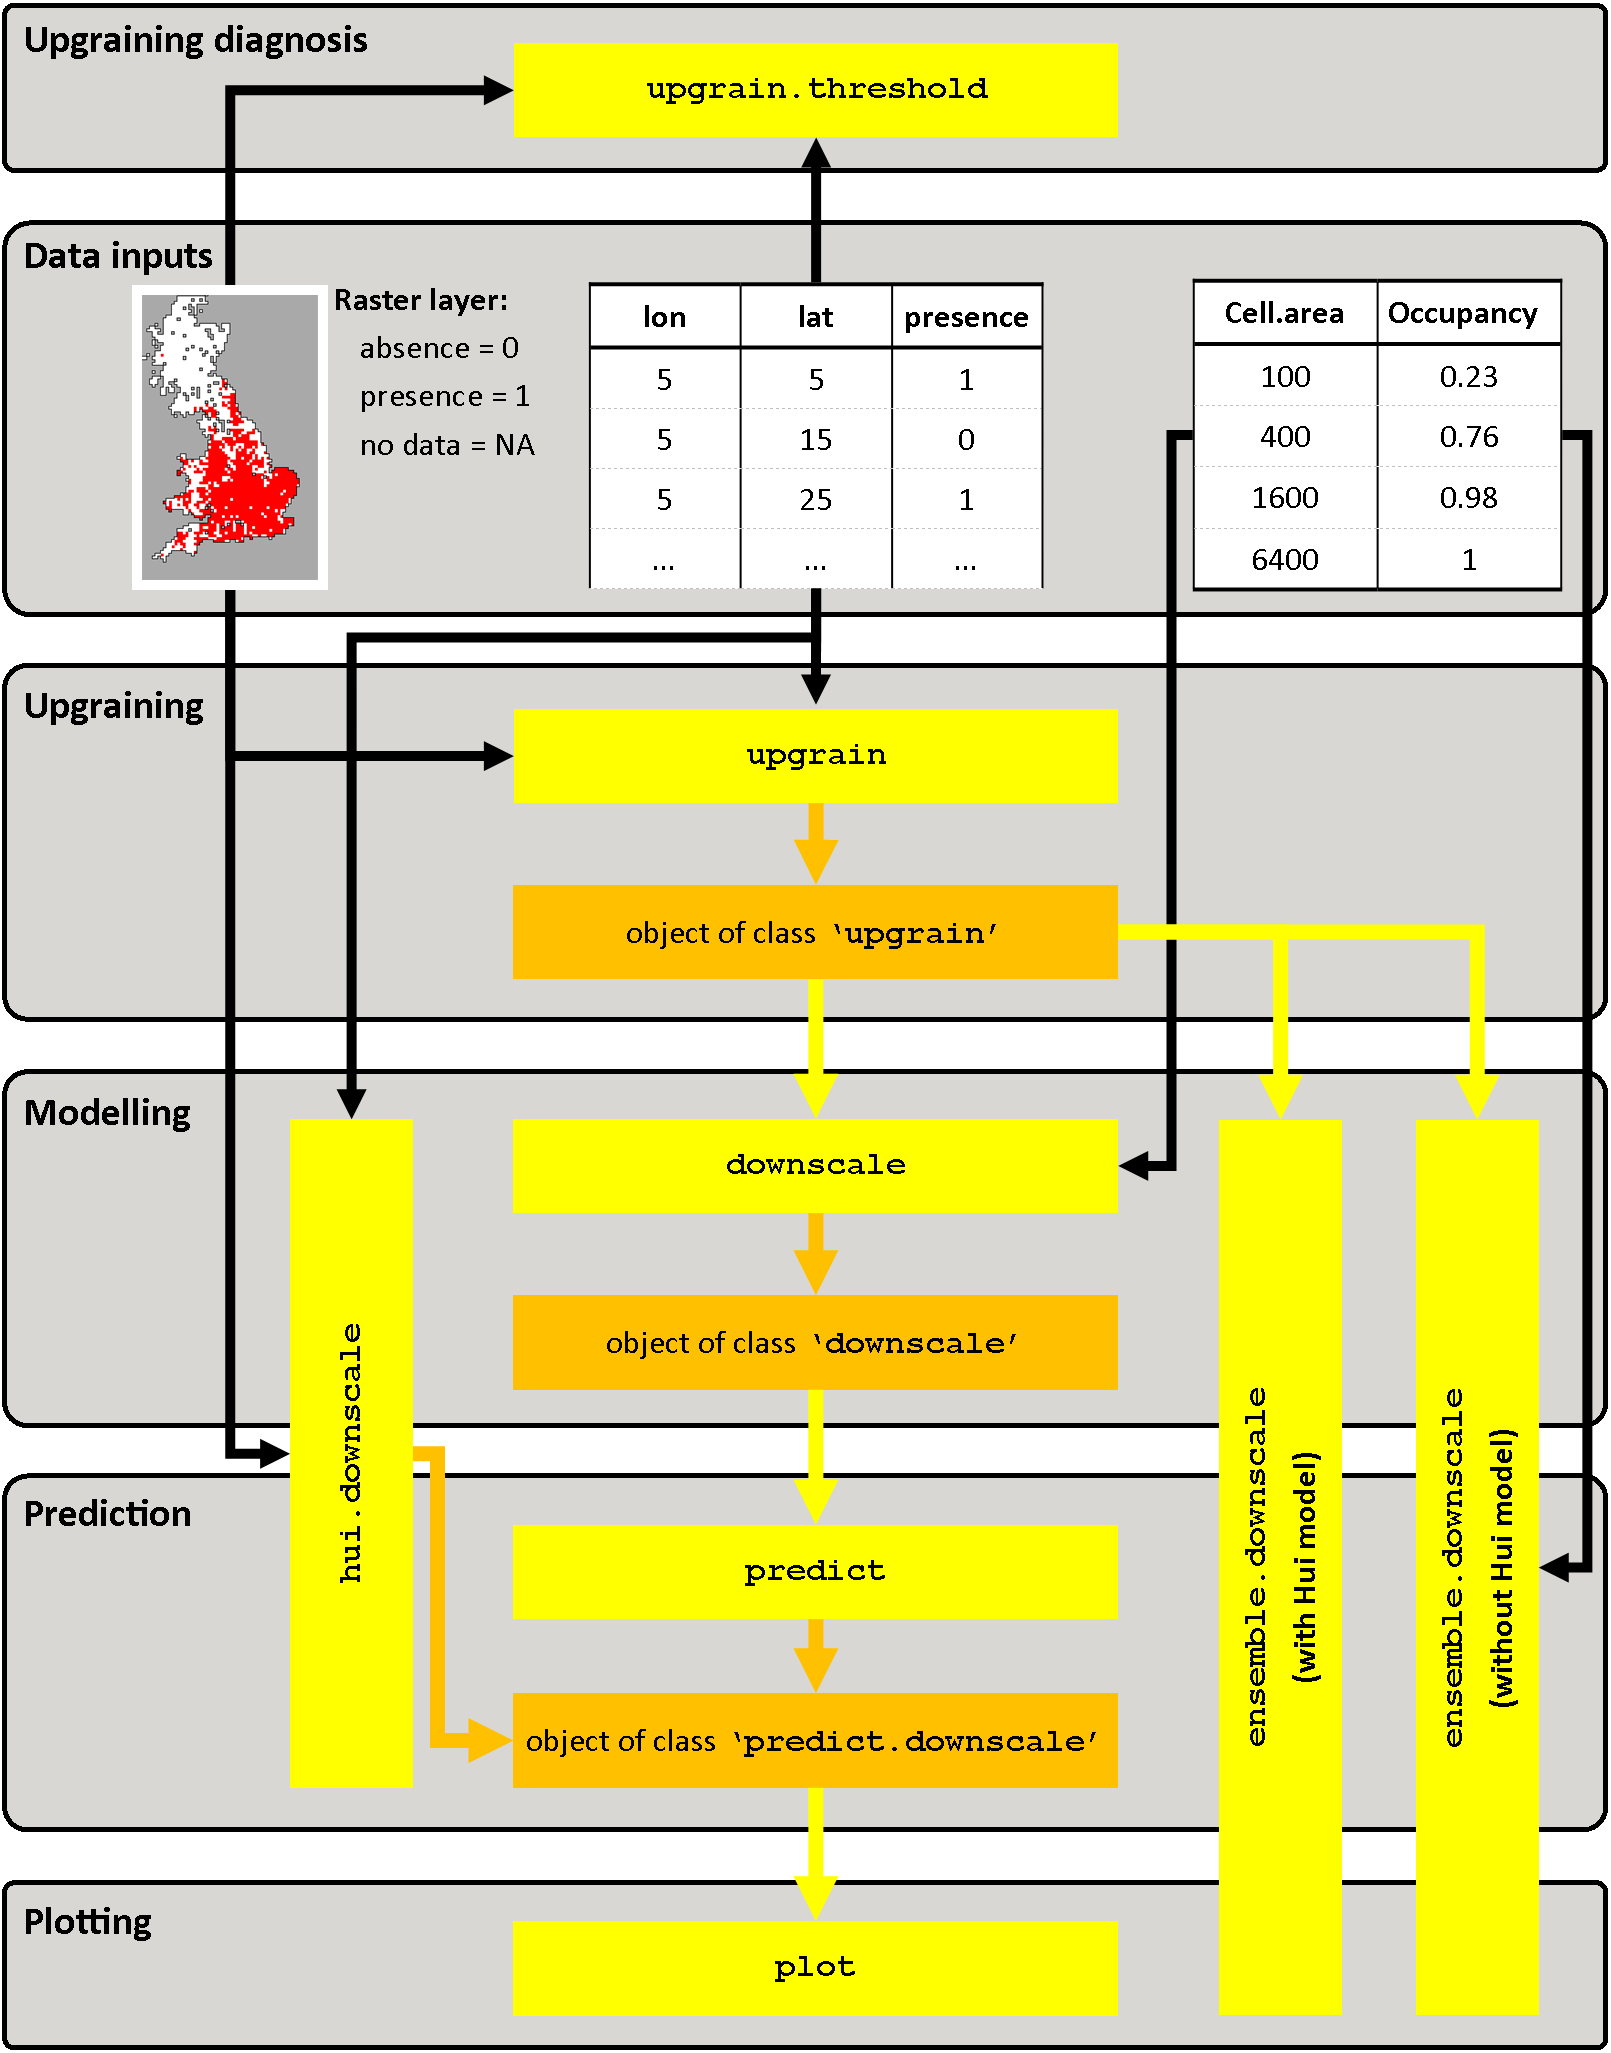
\includegraphics[width=9.9cm]{Flow.png}
\caption{\textbf{Structure of the} \texttt{downscale} \textbf{package showing the flow between the seven functions (yellow) and the three output object classes (orange). Black arrows represent the input of raw data of three types: a raster layer of presence-absence data, a data frame of cell coordinates and presence-absence for each cell, and a data frame of occupancies at coarse-grain sizes. Yellow arrows are where the output of one function may be used as the input for the next function}}
\label{fig:Flow}
\end{figure}

\newpage
To carry out downscaling with the Hui model (Hui et al. 2006, 2009) or upgraining of atlas data (and exploration of upgraining thresholds) then the input data must be of type 2 or 3. The table below shows the functions to use to achieve desired objectives with regards to input data. In all cases \texttt{upgrain.threshold} can be used to explore thresholds for \texttt{upgrain}.

\begin{table}[th]
\small
\centering
\begin{tabular}{| l | l | l |}
\hline
\textbf{Input data type} & \textbf{Objective} & \textbf{Function flow}
\\ \hline
Data frame of cell areas        & Downscale            & $\texttt{downscale} \Rightarrow$ \\ 
and occcupancies                & (excluding Hui model)& $\texttt{predict} \Rightarrow$ \\
                                &                      & $\texttt{plot}$ \\ \hline
Data frame of cell coordinates  & Downscale            & $\texttt{upgrain} \Rightarrow$ \\
and presence-absence data       & (excluding Hui model)& $\texttt{downscale} \Rightarrow$ \\
                                &                      & $\texttt{predict} \Rightarrow$ \\
                                &                      & $\texttt{plot}$ \\ \hline
Raster layer of presence-       & Downscale            & $\texttt{upgrain} \Rightarrow$ \\
absence data                    & (excluding Hui model)& $\texttt{downscale} \Rightarrow$ \\
                                &                      & $\texttt{predict} \Rightarrow$ \\
                                &                      & $\texttt{plot}$ \\ \hline
Data frame of cell coordinates  & Downscale            & ($\texttt{upgrain} \Rightarrow$) \\
and presence-absence data       &	(including Hui model)& $\texttt{hui.downscale} \Rightarrow$ \\
                                &                      & $\texttt{plot}$ \\ \hline
Raster layer of presence-       & Downscale            & ($\texttt{upgrain} \Rightarrow$) \\
absence data                    &	(including Hui model)& $\texttt{hui.downscale} \Rightarrow$ \\
                                &                      & $\texttt{plot}$ \\ \hline
Data frame of cell areas        & Ensemble modelling   & $\texttt{ensemble.downscale}$ \\
and occcupancies                &	(excluding Hui model)& \\ \hline	
Data frame of cell coordinates  & Ensemble modelling   & $\texttt{upgrain} \Rightarrow$ \\
and presence-absence data       &	(with or without Hui model)& $\texttt{ensemble.downscale}$ \\ \hline
Raster layer of presence-       & Ensemble modelling   & $\texttt{upgrain} \Rightarrow$ \\
absence data                    &	(with or without Hui model)& $\texttt{ensemble.downscale}$ \\ \hline
\end{tabular}
\end{table}

For downscale modelling it is important to check the data for the scale of saturation and endemism. The scale of saturation is the grain size where all cells are occupied (fig. \ref{fig:Saturation}a) ie the proportion of occupancy = 1. The scale of endemism is the grain size where all presences occur in a single cell (\ref{fig:Saturation}b). All data above these grain sizes should be discarded as they provide no further information for modelling the occupancy-area curve. The downscale functions will automatically set these occupancies to NA for modelling purposes, but this may lead to insufficient scales remaining for modelling (occupancies for at least three grain sizes are required).

\begin{figure}[!h]
\centering
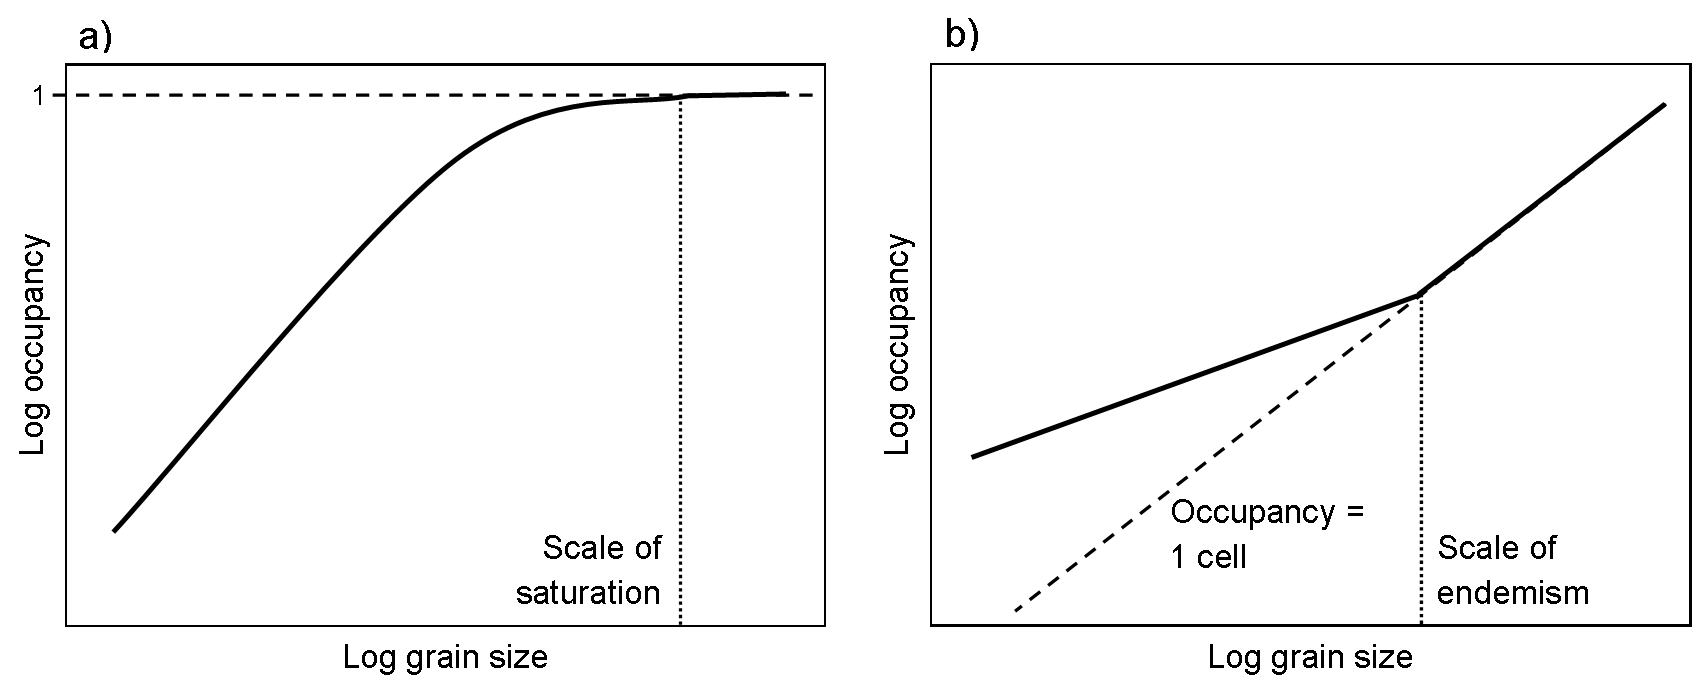
\includegraphics[width=12.5cm]{Saturation.png}
\caption{\textbf{Occupancy-area relationships (OAR) for two species showing a) the scale of saturation (the grain size at which all cells are occupied) and b) the scale of endemism (the scale at which only one cell is occupied).}}
\label{fig:Saturation}
\end{figure}

\newpage
\section{Package tutorial}

First, we must download the downscale package from CRAN if not already done so.

\begin{Schunk}
\begin{Sinput}
install.packages("downscale")
\end{Sinput}
\end{Schunk}

Then load in the library

\begin{Schunk}
\begin{Sinput}
library("downscale")
\end{Sinput}
\end{Schunk}

\subsection{A quick example}
We will start with the simplest example of using the downscaling package, where we already have occupancy data across a number of grain sizes. We first create some dummy data; a data frame where the first column are the cell areas (grain size) and the proportion of occupancy as the second column:

\begin{Schunk}
\begin{Sinput}
occupancy <- data.frame(Cell.area = c(100, 400, 1600, 6400),
                        Occupancy = c(0.23, 0.56, 0.87, 1))
\end{Sinput}
\end{Schunk}

Now we use downscale to estimate the model parameters for the logistic model to the data. Note: for this type of data input we must also specify the extent (the total area over which occupancy has been measured) which is necessary for converting the modelled proportion of occupancies to area of occupancy (AOO) later on. In this dummy data we will set extent to be 320000 km$^2$:

\begin{Schunk}
\begin{Sinput}
## fit logistic model to observed data using downscale
logis.mod <- downscale(occupancies = occupancy,
                       model = "Logis",
                       extent = 320000)
                       
## this creates an object of class ‘downscale’
logis.mod
\end{Sinput}
\begin{Soutput}
$model
[1] "Logis"

$pars
          C           z 
0.002014927 1.083725424 

$observed
  Cell.area Occupancy
1       100      0.23
2       400      0.56
3      1600      0.87
4      6400      1.00

$extent
[1] 320000

attr(,"class")
[1] "downscale"

\end{Soutput}
\end{Schunk}

The downscale function has estimated best-fit parameters of 0.00201 for \texttt{C} and 1.0837 for \texttt{z} for the logistic model. We then take these parameters from the \texttt{‘downscale’} object to extrapolate the fitted logistic function to predict occupancies at finer grain sizes. We will first create a vector of grain sizes (cell area) to predict. If we include the original cell sizes used for modelling we can also observe the model fit.

\begin{Schunk}
\begin{Sinput}
## new grain sizes to predict
areas.pred <- c(1, 2, 5, 25, 100, 400, 1600, 6400)

## predict for the new grain sizes using the downscale object
logis.pred <- predict(logis.mod,
                      new.areas = areas.pred,
                      plot = FALSE)
                      
## this creates an object of class ‘predict.downscale’
## occupancy is given as a proportion (Occupancy) and area of occupancy (AOO)
logis.pred$predicted
\end{Sinput}
\begin{Soutput}
  Cell.area   Occupancy         AOO
1         1 0.002010876    643.4802
2         2 0.004252482   1360.7942
3         5 0.011396541   3646.8932
4        25 0.061873397  19799.4871
5       100 0.228564935  73140.7793
6       400 0.570999511 182719.8435
7      1600 0.856717834 274149.7068
8      6400 0.964106833 308514.1867
\end{Soutput}
\end{Schunk}
\begin{Schunk}
\begin{Sinput}
## now we can plot the predictions with log-log axes.
## Black points are the observed values, red points are the predicted values
plot(logis.pred)
\end{Sinput}
\end{Schunk}
{\centering 
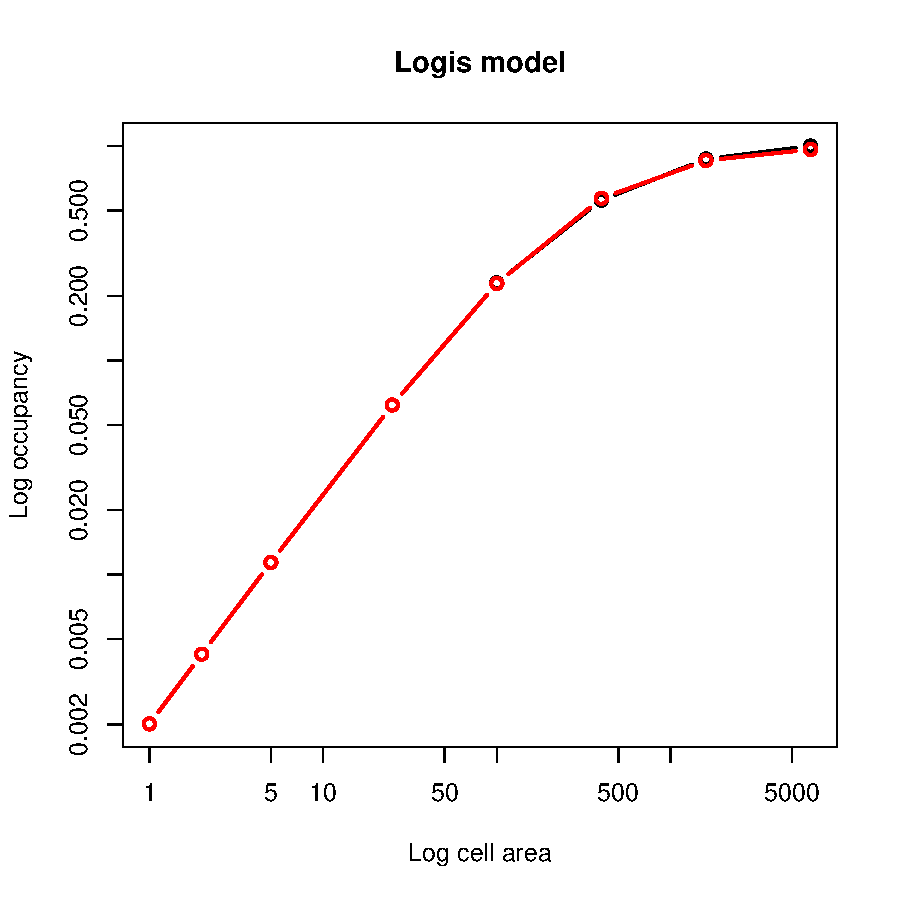
\includegraphics[width=9cm]{Downscaling-downscale6} \par
}

\subsection{Preparing atlas data for downscaling}
For the majority of cases we will have atlas data. For downscaling we will need to therefore upgrain the atlas data. Read in the atlas data for a hypothetical UK species provided in the package. In this case the format is a data frame of sample cell coordinates and presence-absence data:

\begin{Schunk}
\begin{Sinput}
## if it is not already loaded, load in the package
library(downscale)
data.file <- system.file("extdata", "atlas_data.txt", package = "downscale")
atlas.data <- read.table(data.file, header = TRUE)
\end{Sinput}
\end{Schunk}

The data frame must have the column names “lon”, “lat” and “presence”:

\begin{Schunk}
\begin{Sinput}
head(atlas.data)
\end{Sinput}
\begin{Soutput}
   lon lat presence
1 8170  10        0
2 8130  20        0
3 8140  20        0
4 8160  20        0
5 8170  20        0
6 8140  30        0
\end{Soutput}
\end{Schunk}

The first step is to upgrain the atlas data to calculate occupancy at larger grain sizes than the atlas data – this provides the occupancy data points to fit the different downscaling models to. If we simply increase the cell sizes of the atlas data then the extent also increases. As downscaling models requires the proportion of occupancy at each grain, if the proportions are calculated from a different total area in each case we may run in to problems. Therefore it is important that we fix the extent of all grain sizes to the extent of the largest grain size, but this means compromising between assigning unsampled cells as absences or excluding sampled cells.

It is highly recommended to read the vignette “Upgraining atlas data for downscaling: threshold selection using upgrain.threshold” for more detail on creating your multi-scale standardised atlas data, as well as the help file for the \texttt{upgrain.threshold} function:

\begin{Schunk}
\begin{Sinput}
vignette("Upgraining", package = "downscale")
?upgrain.threshold
\end{Sinput}
\end{Schunk}

The \texttt{upgrain.threshold} allows the user to explore these trade-offs through several plots, and also provides four recommendations for possible threshold selections: including all sampled cells; including only cells at the largest grain size that were completely sampled at the atlas scale; a species-specific threshold that retains all species occurrences; and an atlas-specific threshold that maintains the same extent as the original atlas data. As the input data is a data frame we must tell the function the cell width (10 km$^2$) and the number of scales we wish to upgrain (we want three additional scales for modelling):

\begin{Schunk}
\begin{Sinput}
## explore thresholds using upgrain.threshold
thresh <- upgrain.threshold(atlas.data = atlas.data,
                            cell.width = 10,
                            scales = 3,
                            thresholds = seq(0, 1, 0.01))
\end{Sinput}
\end{Schunk}

This gives two sets of plots. The first are a set of four plots that explore the trade-offs between discarding sampled cells and making assumptions about unsampled cells, which are automatically assigned as absences.

\newpage
\begin{figure}[!h]
\centering
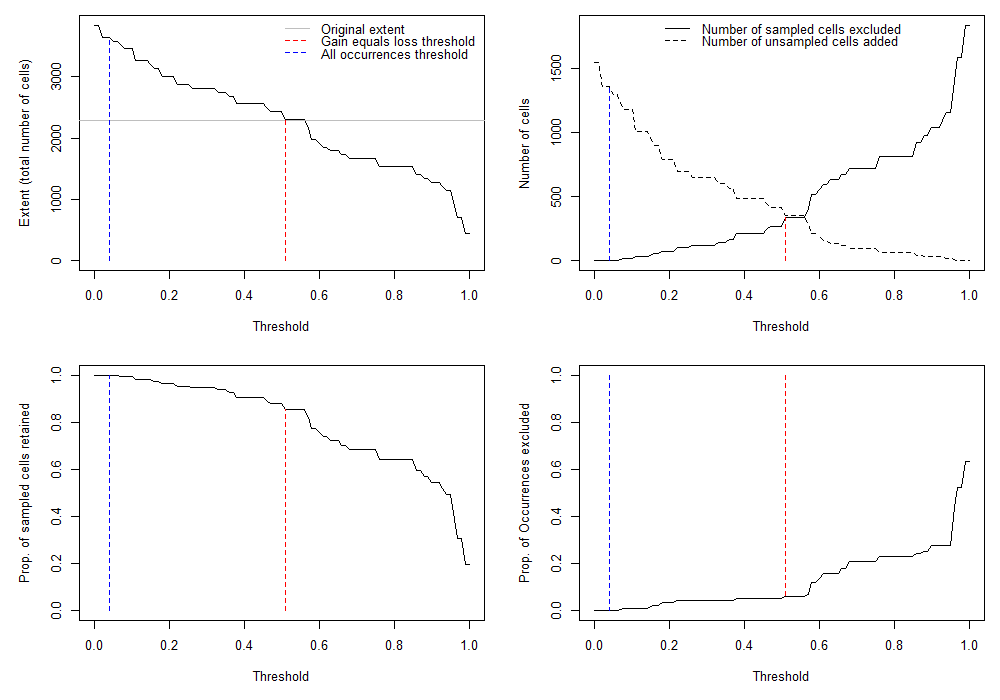
\includegraphics[width=12.5cm]{Threshold_plots.png}
\end{figure}

The second set of plots (hit \texttt{return} or click on the plot window to view the second window) are the standardised atlas data generated after applying the four different threshold criteria ("All Sampled",  "All Occurrences",  "Gain Equals Loss" and "Sampled Only").

\begin{figure}[!h]
\centering
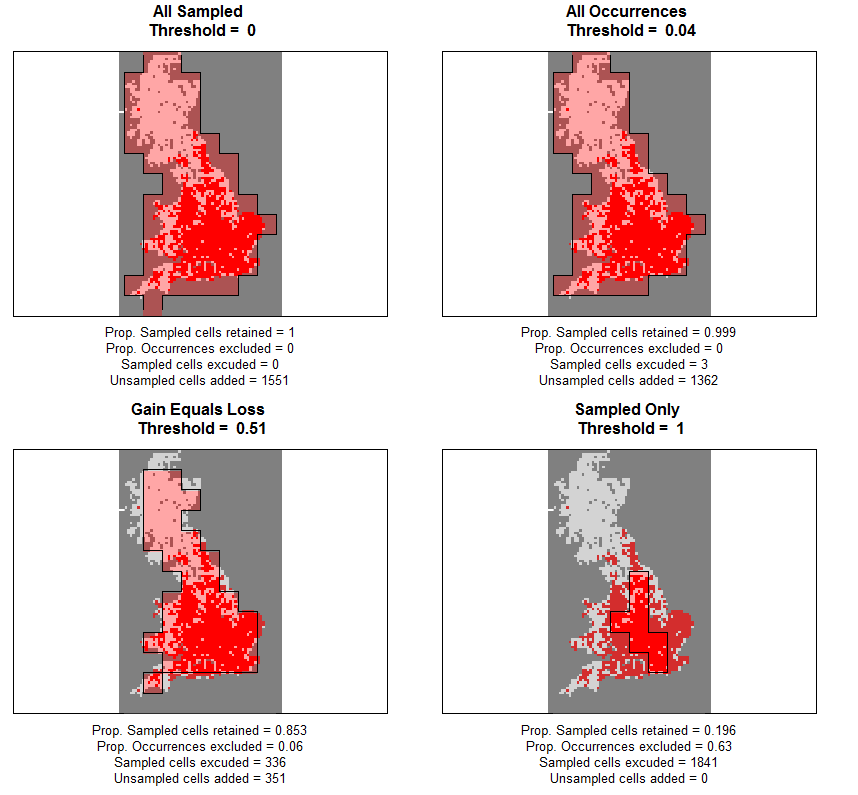
\includegraphics[width=12cm]{Threshold_maps.png}
\end{figure}

We can see the threshold values for the four threshold criteria

\begin{Schunk}
\begin{Sinput}
thresh$Thresholds
\end{Sinput}
\begin{Soutput}
  All_Sampled All_Occurrences Gain_Equals_Loss Sampled_Only
1           0            0.04             0.51            1
\end{Soutput}
\end{Schunk}

Once the user has decided on a threshold value (any value between 0 and 1 can be selected) or one of the threshold criteria, the \texttt{upgrain} function will prepare the atlas data for downscaling. For now we’ll use one of the pre-defined options “All\_Occurrences” which ensures that all occurrence records are retained. This creates an object of class \texttt{‘upgrain’} which can then then be used directly as an input for \texttt{downscale}, along with plots of the original and standardised atlas data at each scale.

\begin{Schunk}
\begin{Sinput}
## upgrain data (using All Occurrences threshold)
occupancy <- upgrain(atlas.data,
                     cell.width = 10,
                     scales = 3,
                     method = "All_Occurrences",
                     plot = TRUE)
\end{Sinput}
\end{Schunk}
\begin{figure}[!h]
\centering
\includegraphics[width=12.5cm]{Downscaling-downscale11}
\end{figure}

\subsection{Downscaling the atlas data - more detailed examples}

As we can pass our \texttt{‘upgrain’} directly in to \texttt{‘downscale’} we no longer require to specify the extent. Let’s try the improved negative binomial model (INB) first:

\begin{Schunk}
\begin{Sinput}
## Improved Negative Binomial model
(inb <- downscale(occupancies = occupancy,
                  model = "INB"))
\end{Sinput}
\begin{Soutput}
$model
[1] "INB"

$pars
         C          r          b 
1.42670491 0.04906771 1.82970792 

$observed
  Cell.area Occupancy
1       100 0.2713542
2       400 0.4122807
3      1600 0.5219298
4      6400 0.7017544

$extent
[1] 364800

attr(,"class")
[1] "downscale"

\end{Soutput}
\end{Schunk}

The downscaling functions use an optimisation procedure to fit the models to the upgrained occupancy data. Suitable starting values for model parameters are automatically inputted, however if the models aren’t converging then it is possible to specify user-specific parameters. The table below shows the default starting parameters implemented.

\begin{table}[!ht]
\centering
\begin{tabular}{| l | l | l | l |}
\hline
\textbf{Model} & \textbf{Parameter 1} &	\textbf{Parameter 2} &	\textbf{Parameter 3} \\\hline
\texttt{Nachman}  &	\texttt{"C"} = 0.01       &	\texttt{"z"} = 0.01 & \\	
\texttt{PL}       &	\texttt{"C"} = 0.01       &	\texttt{"z"} = 0.01 & \\
\texttt{Logis}    &	\texttt{"C"} = 0.01       &	\texttt{"z"} = 0.01 & \\	
\texttt{Poisson}  &	\texttt{"lambda"} = 1e-8  &  &	\\
\texttt{NB}       &	\texttt{"C"} = 0.01       &	\texttt{"k"} = 0.01 & \\	
\texttt{GNB}	    & \texttt{"C"} = 0.00001    &	\texttt{"z"} = 1    &	\texttt{"k"} = 0.01 \\
\texttt{INB}	    & \texttt{"C"} = 1          &	\texttt{"r"} = 0.01 &	\texttt{"b"} = 0.1 \\
\texttt{FNB}	    & \texttt{"W"} = 10         &	\texttt{"k"} = 10   & \\	
\texttt{Thomas}   &	\texttt{"rho"} = 1e-8     &	\texttt{"mu"} = 10  &	\texttt{"sigma"} = 1 \\\hline
\end{tabular}
\label{table:pars}
\end{table}

If using your own parameters, they must be in the form of a list with the same parameter names (take particular note of capitals) as the original starting parameters:

\begin{Schunk}
\begin{Sinput}
## Specifying the starting parameters
params.new <- list("C" = 0.1, "r" = 0.00001, "b" = 0.1)
inb.new <- downscale(occupancies = occupancy,
                     model = "INB",
                     starting_params = params.new)
\end{Sinput}
\end{Schunk}

We can visually compare the two to see which has a better fit by extrapolating the modelled curves to finer grain sizes using \texttt{predict} as before (plotting can be called directly from \texttt{predict} or through \texttt{plot}). The first plot is the prediction using the original parametersm and the second plot using the new parameters (a much worse fit in this case):

\begin{Schunk}
\begin{Sinput}
## plot the predictions of two FNB models using predict.downscale
inb.pred <- predict(inb,
                    new.areas = c(1, 2, 5, 25, 100, 400, 1600, 6400),
                    plot = TRUE)
inb.pred.new <- predict(inb.new,
                        new.areas = c(1, 2, 5, 25, 100, 400, 1600, 6400),
                        plot = TRUE)
\end{Sinput}
\end{Schunk}
\begin{figure}[!h]
\centering
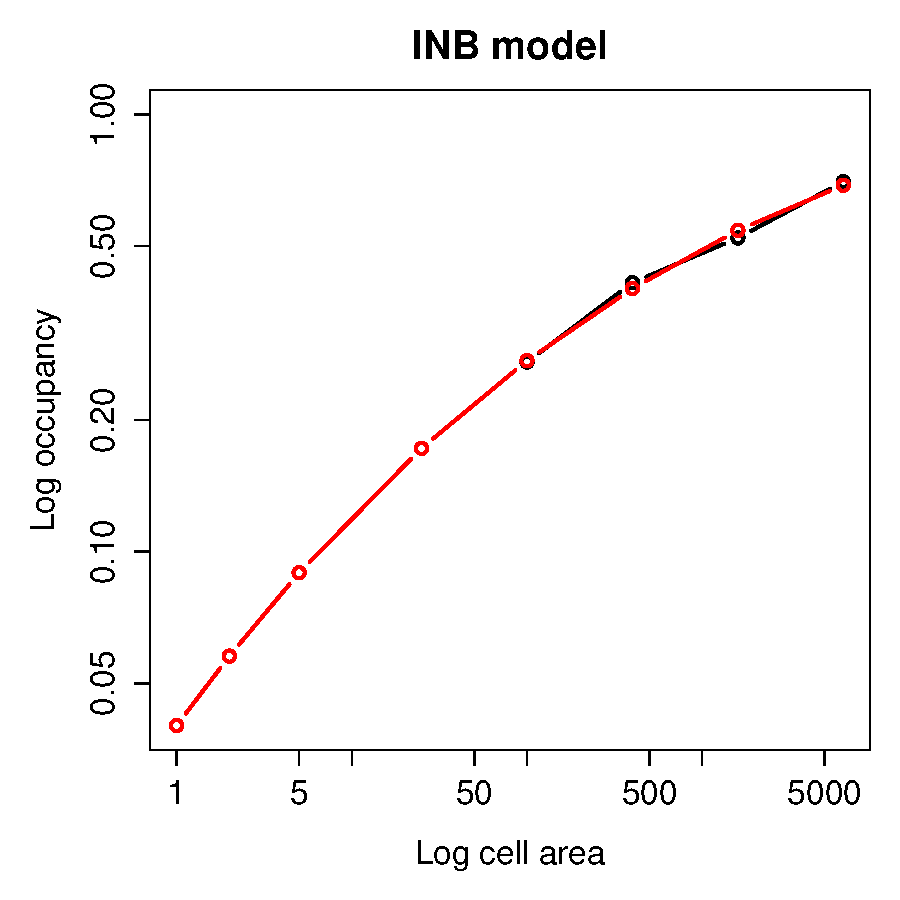
\includegraphics[width=7cm]{Downscaling-downscale13}
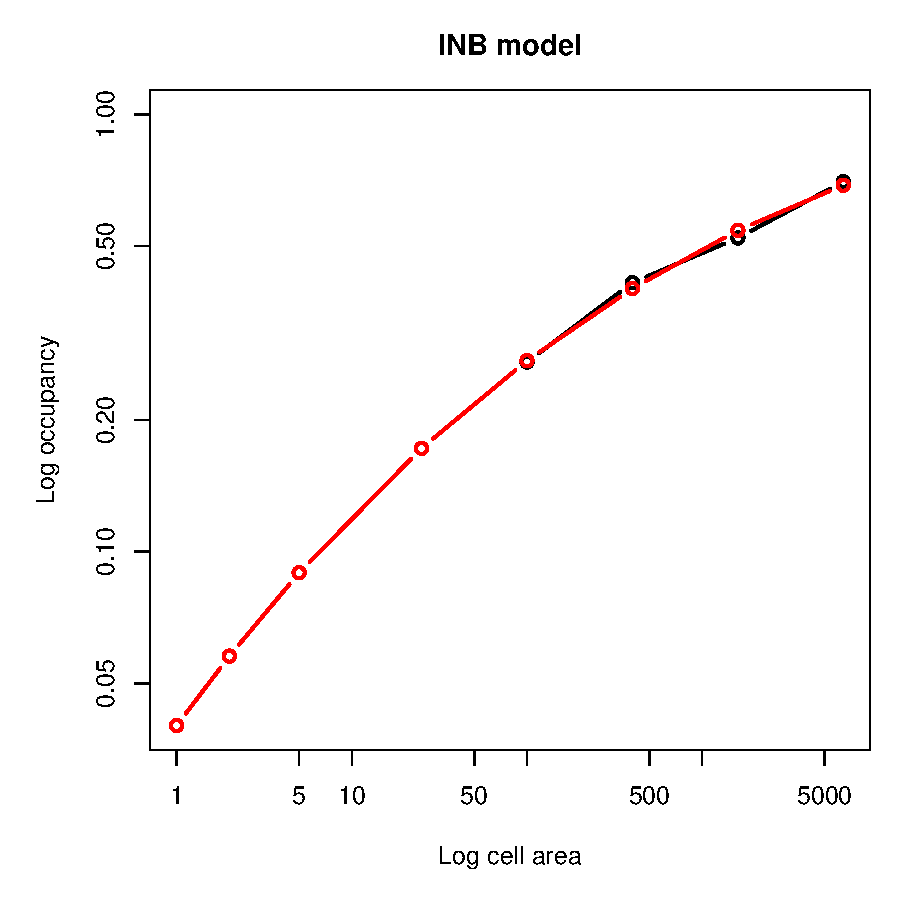
\includegraphics[width=7cm]{Downscaling-downscale14}
\end{figure}


The Thomas model involves an integration process that can be time-consuming to run. For this reason the user may alter the tolerance during integration – the finer the tolerance the more accurate the prediction but the longer the computation time. It can therefore be a good idea to initially try a larger tolerance value than the default ($1e^{-6}$) in order to ascertain if the starting parameters are likely to be correct. You can then always then use the parameter esimates as the starting parameters when using a smaller tolerance value.

\begin{Schunk}
\begin{Sinput}
## Thomas model
thomas <- downscale(occupancies = occupancy,
                    model = "Thomas",
                    tolerance = 1e-3)
                    
## the tolerance can also be set for the predict function
thomas.pred <- predict(thomas,
                       new.areas = c(1, 2, 5, 25, 100, 400, 1600, 6400),
                       tolerance = 1e-6)

## When plotting the results we can also change the look of the graphics
plot(thomas.pred,
     col.pred = "green",  # change the colour of the prediction
     pch = 16,            # change point character
     lwd.obs = 3)         # change line width of the observed data
\end{Sinput}
\end{Schunk}
\begin{figure}[!ht]
\centering
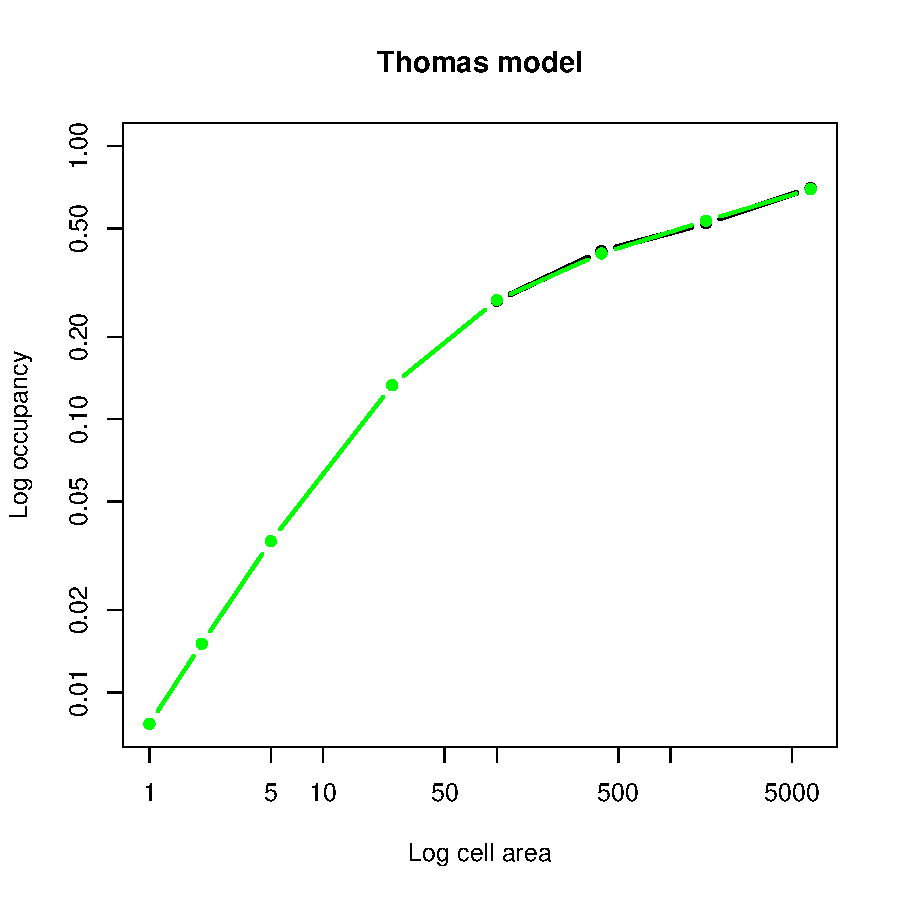
\includegraphics[width=9cm]{Downscaling-downscale16}
\end{figure}

The Hui model is slightly different from the other downscaling models in that it does not need occupancy from multiple scales. Instead, it only takes the coordinates of presence-absence data at the atlas scale and uses this to calculate occupancy at finer grain sizes. For this reason it is implemented using a seperate function, \texttt{hui.downscale}, which in effect runs \texttt{downscale} and \texttt{predict.downscale} in a single step. 

The input data must either be a presence-absence raster layer of the atlas data, or a data frame of cell coordinates and presence-absence data. Additionally the function requires the cell widths of the input data, if using a data frame as the input data, the total extent, and the grain sizes (cell area) for which we wish to predict occupancy. These must be smaller than the cell area of the input data. Like the Thomas model, the tolerance can be specified if the results appear inaccurate (set tolerance to a smaller number) or takes extensive programming time (set tolerance to a larger number).

\begin{Schunk}
\begin{Sinput}
## Hui model using a data frame as input
hui <- hui.downscale(atlas.data,
                     cell.width = 10,
                     extent = 320000,
                     new.areas = c(1, 2, 5, 15, 50))

## the output is a normal ‘predict.downscale’ object	
plot(hui)

## Or we can use the 'upgrain' object as input
hui <- hui.downscale(occupancy,
                     cell.width = 10,
                     extent = 320000,
                     new.areas = c(1, 2, 5, 15, 50),
                     plot = TRUE)
\end{Sinput}
\end{Schunk}
\begin{figure}[!ht]
\centering
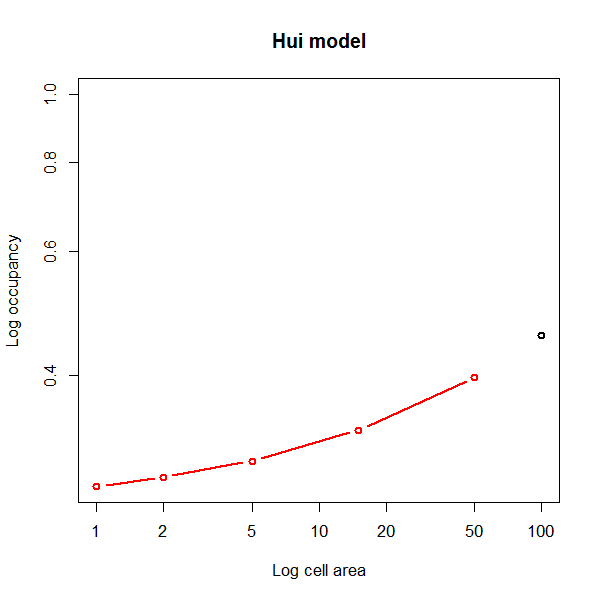
\includegraphics[width=7cm]{Downscaling-downscale18}
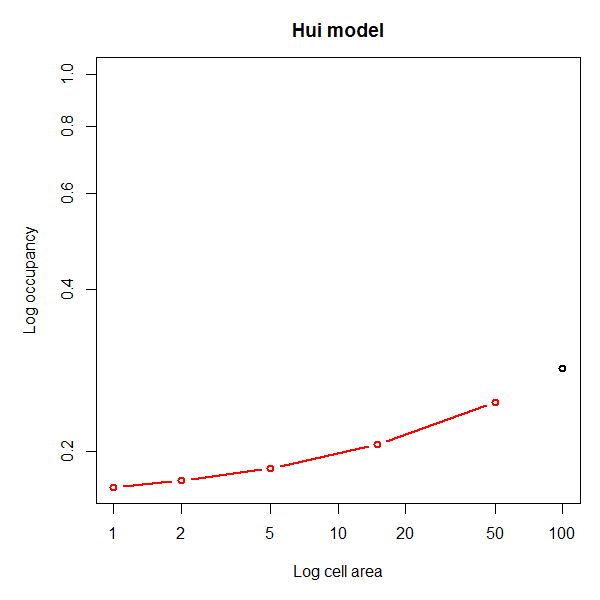
\includegraphics[width=7cm]{Downscaling-downscale19}
\end{figure}

It is critical to note here that the proportion of occupancies are very different between the two plots. This is because the extents are different between the original atlas data 320000 km$^2$ and the standardised atlas data 364800 km$^2$. If comparing predictions using multiple models it is crucial to use the same standardised data in all cases, or else only compare the converted area of occupancies (AOO), not proportion of occupancies.

\subsection{Ensemble modelling}
No single model appears to provide the most accurate fine-scale occupancy predictions in all cases, and it is difficult to predict which model will in a given situation. The ensemble function will model and predict occupancy for multiple models simultaneously, and also applies a simple model averaged prediction (the means of the log occupancies). Some or all of the models can be selected. Again, lets start where our data is a data frame of occupancies at each grain size:

\begin{Schunk}
\begin{Sinput}
## hypothetical occupancy data
occupancy <- data.frame(Cell.area = c(100, 400, 1600, 6400),
                        Occupancy = c(0.23, 0.56, 0.87, 1))
                        
## grain sizes (cell areas) to predict
areas.pred <- c(1, 2, 5, 25, 100, 400, 1600, 6400)
\end{Sinput}
\end{Schunk}

The \texttt{ensemble.downscale} function does the modelling and predicting in a single step so we need a few more arguments than when just using \texttt{downscale}: the cell areas of the fine grain sizes we wish to predict, the total extent and the models we wish to apply. Also note, with this type of input data we can not apply the Hui model.

\begin{Schunk}
\begin{Sinput}
ensemble <- ensemble.downscale(occupancy,
                               new.areas = areas.pred,
                               extent = 320000,
                               models = c("Nachman",
                                          "PL",
                                          "Logis",
                                          "GNB",
                                          "FNB"),
                               plot = TRUE)
\end{Sinput}
\begin{Soutput}
Nachman model is running...  complete 
PL model is running...  complete 
Logis model is running...  complete 
GNB model is running...  complete 
FNB model is running...  complete 
\end{Soutput}
\end{Schunk}

\begin{figure}[!ht]
\centering
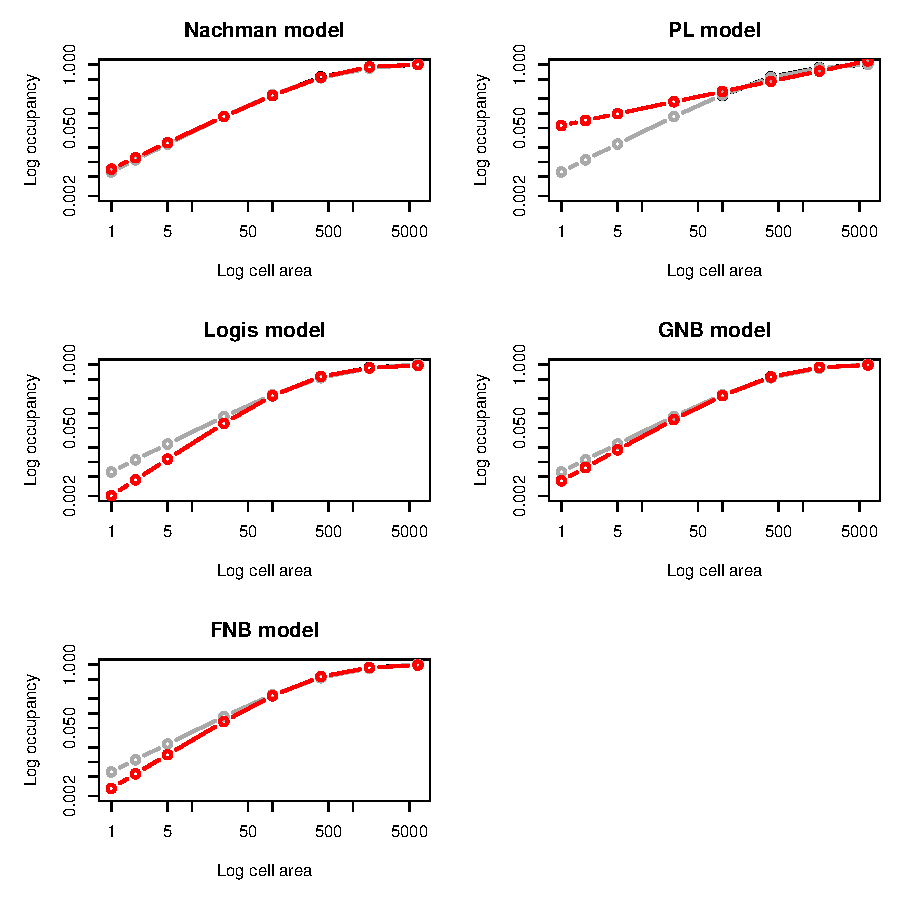
\includegraphics[width=13cm]{Downscaling-downscale}
\end{figure}

\begin{Schunk}
\begin{Sinput}
## the model averaged predictions are in grey
## to print the predicted proportion of occupancies for each model
ensemble$Occupancy
\end{Sinput}
\begin{Soutput}
  Cell.area    Nachman        PL      Logis        GNB        FNB      Means
1         1 0.00708498 0.0558199 0.00201088 0.00405949 0.00284089 0.00620137
2         2 0.01217964 0.0711372 0.00425248 0.00764569 0.00566805 0.01098108
3         5 0.02485181 0.0980179 0.01139654 0.01758727 0.01406806 0.02330096
4        25 0.08522024 0.1721162 0.06187339 0.07373553 0.06710741 0.08520463
5       100 0.23247468 0.2795353 0.22856494 0.23018897 0.22857598 0.23910431
6       400 0.54430571 0.4539953 0.57099951 0.55812208 0.56665466 0.53692736
7      1600 0.90314840 0.7373372 0.85671783 0.87738733 0.87016143 0.84685851
8      6400 0.99902662 1.1975149 0.96410683 0.98448699 0.97632517 1.02083964
\end{Soutput}
\begin{Sinput}


## and print the predicted area of occupancies (AOO) for each model
ensemble$AOO
\end{Sinput}
\begin{Soutput}
  Cell.area    Nachman        PL       Logis        GNB         FNB      Means
1         1   2267.193  17862.39    643.4802   1299.035    909.0862   1984.439
2         2   3897.484  22763.91   1360.7942   2446.623   1813.7772   3513.945
3         5   7952.579  31365.75   3646.8932   5627.925   4501.7776   7456.307
4        25  27270.478  55077.20  19799.4871  23595.370  21474.3707  27265.480
5       100  74391.897  89451.29  73140.7793  73660.469  73144.3146  76513.378
6       400 174177.827 145278.51 182719.8435 178599.064 181329.4907 171816.756
7      1600 289007.489 235947.91 274149.7068 280763.946 278451.6571 270994.723
8      6400 319688.520 383204.78 308514.1867 315035.837 312424.0534 326668.684
\end{Soutput}
\end{Schunk}

Alternatively, the input data may be an object of class \texttt{‘upgrain’}, which also allows us to run the Hui model as long as we specify the cell width:

\begin{Schunk}
\begin{Sinput}
## read in atlas data
data.file <- system.file("extdata", "atlas_data.txt", package = "downscale")
atlas.data <- read.table(data.file, header = TRUE)
\end{Sinput}
\end{Schunk}
\setkeys{Gin}{width=1\linewidth}
\begin{Schunk}
\begin{Sinput}
## upgrain data (using All Occurrences threshold)
occupancy <- upgrain(atlas.data,
                     cell.width = 10,
                     scales = 3,
                     method = "All_Occurrences",
                     plot = FALSE)

## ensemble modelling
ensemble <- ensemble.downscale(occupancy,
                               new.areas = areas.pred,
                               cell.width = 10,
                               models = c("Nachman",
                                          "PL",
                                          "Logis",
                                          "GNB",
                                          "FNB",
                                          "Hui"),
                              plot = TRUE)
\end{Sinput}
\begin{Soutput}
Nachman model is running...  complete 
PL model is running...  complete 
Logis model is running...  complete 
GNB model is running...  complete 
FNB model is running...  complete 
Hui model is running...  complete 
\end{Soutput}
\end{Schunk}

\begin{figure}[!ht]
\centering
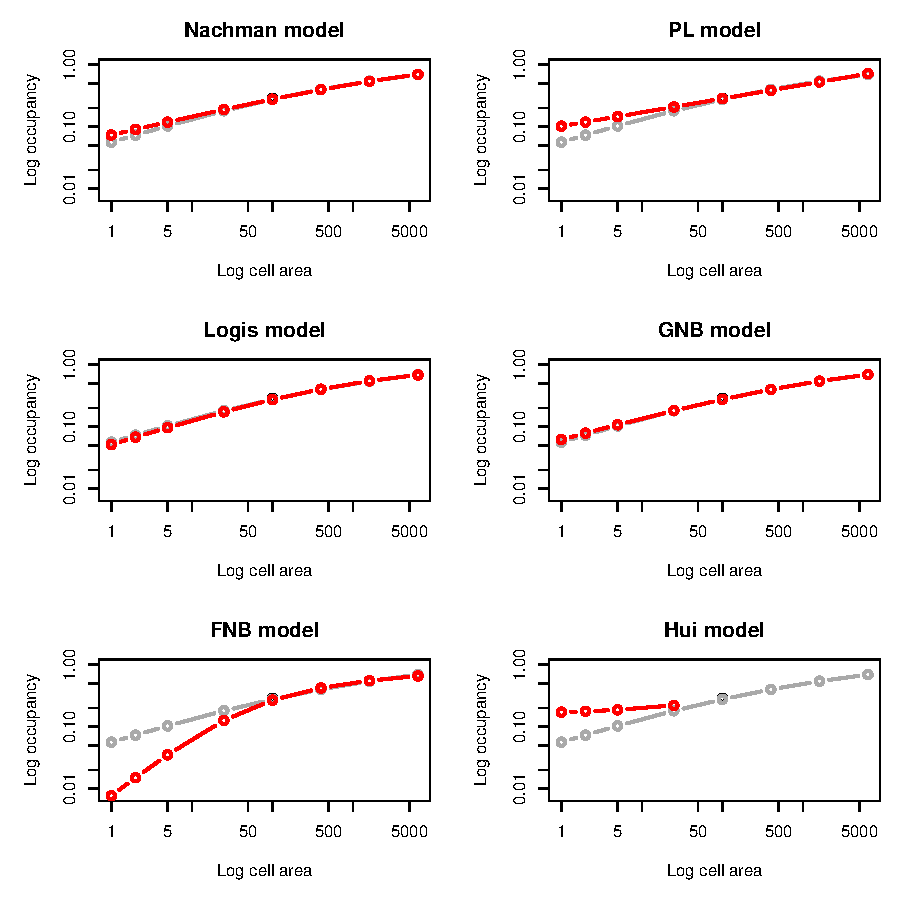
\includegraphics[width=13cm]{Downscaling-downscale23}
\end{figure}

\newpage
If we want to run all ten models we can specify \texttt{models = "all"}. Once again, we can set the tolerance values for the modelling (\texttt{tolerance\_mod}) and prediction (\texttt{tolerance\_pred}) of the Thomas model and the Hui model (\texttt{tolerance\_hui}) to improve processing times or accuracy.

\begin{Schunk}
\begin{Sinput}
ensemble <- ensemble.downscale(occupancy,
                               new.areas = areas.pred,
                               cell.width = 10,
                               models = "all",
                               tolerance_mod = 1e-3,
                               plot = TRUE)
\end{Sinput}
\begin{Soutput}
Nachman model is running...  complete 
PL model is running...  complete 
Logis model is running...  complete 
Poisson model is running...  complete 
NB model is running...  complete 
GNB model is running...  complete 
INB model is running...  complete 
FNB model is running...  complete 
Thomas model is running...  complete 
Hui model is running...  complete 
\end{Soutput}
\end{Schunk}

\begin{figure}[!ht]
\centering
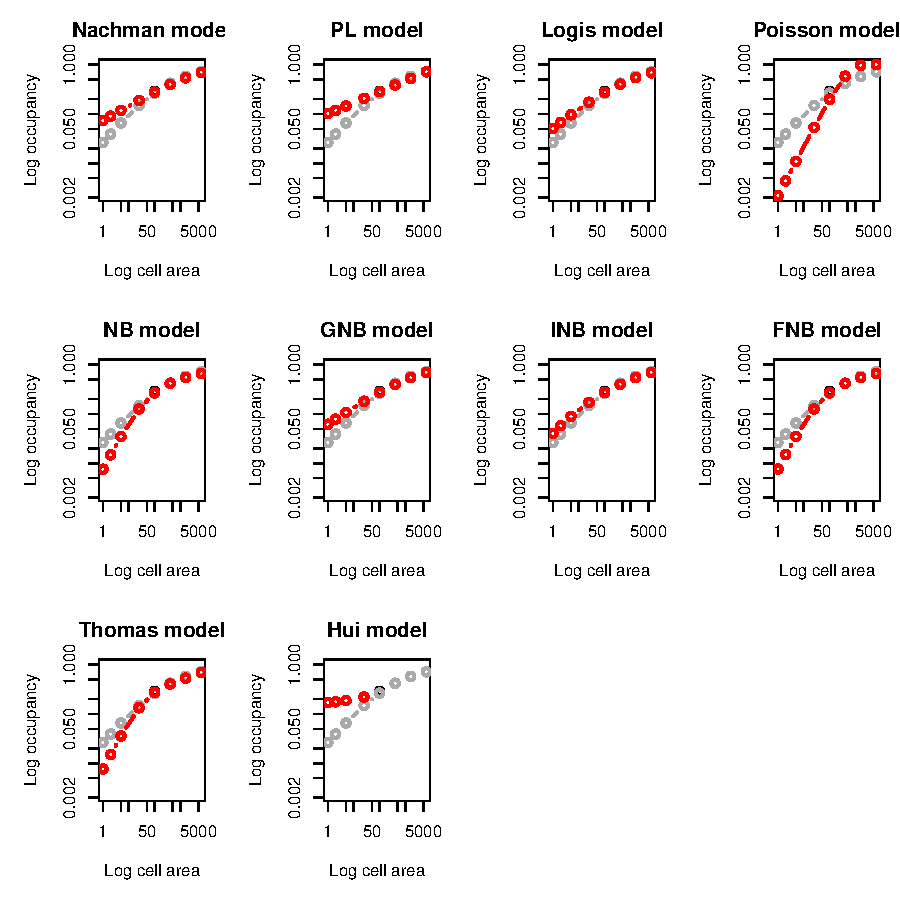
\includegraphics[width=\linewidth]{Downscaling-downscale24}
\end{figure}

We can also specify the starting parameters for specific models. For each model the starting parameters should be in the form of a list as before, and each model list is an item in a combined list:

\begin{Schunk}
\begin{Sinput}
## Specifying starting parameters for Nachman and GNB models
new.params <- list(Nachman = list("C" = 0.1, "z" = 0.01),
                   GNB = list("C" = 0.1, "z" = 1, "k" = 0.01))
new.params
\end{Sinput}
\begin{Soutput}
$Nachman
$Nachman$C
[1] 0.1

$Nachman$z
[1] 0.01


$GNB
$GNB$C
[1] 0.1

$GNB$z
[1] 1

$GNB$k
[1] 0.01


\end{Soutput}
\end{Schunk}

\begin{Schunk}
\begin{Sinput}
ensemble <- ensemble.downscale(occupancies = occupancy,
                               new.areas = c(1, 2, 5, 15, 50, 100, 400, 1600,
                                             6400),
                               cell.width = 10,
                               models = "all",
                               tolerance_mod = 1e-3,
                               starting_params = new.params,
                               plot = TRUE)
\end{Sinput}
\begin{Soutput}
Nachman model is running...  complete 
PL model is running...  complete 
Logis model is running...  complete 
Poisson model is running...  complete 
NB model is running...  complete 
GNB model is running...  complete 
INB model is running...  complete 
FNB model is running...  complete 
Thomas model is running...  complete 
Hui model is running...  complete 

\end{Soutput}
\end{Schunk}

\begin{figure}[!ht]
\centering
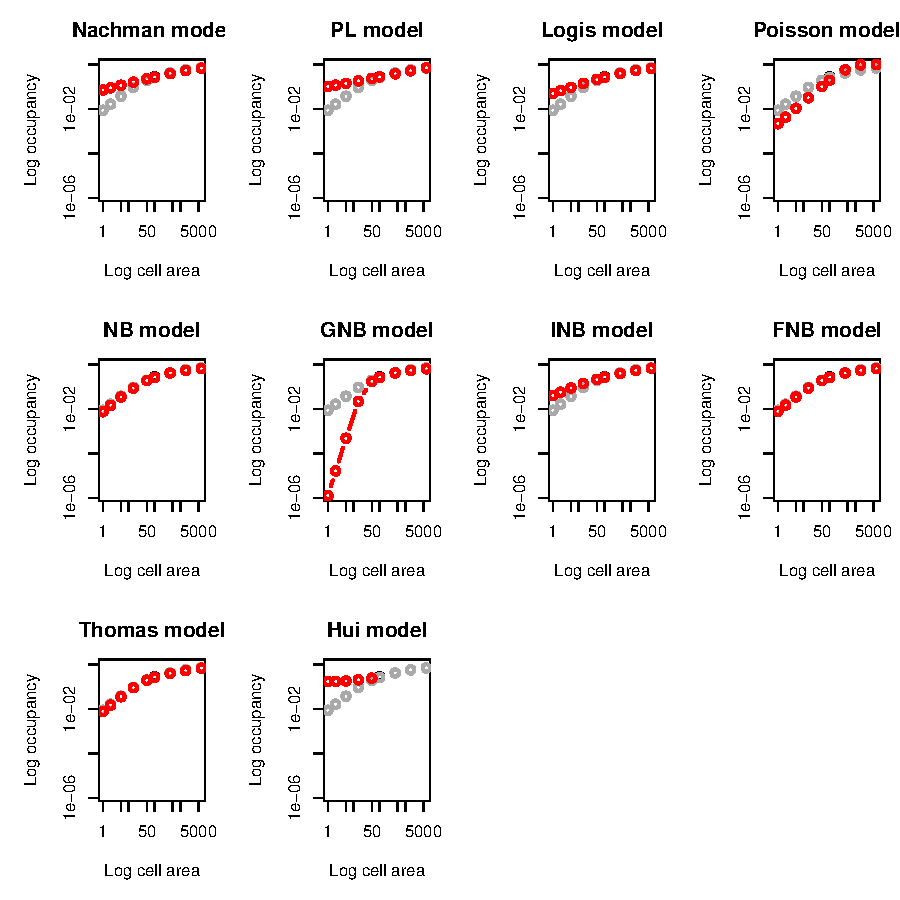
\includegraphics[width=\linewidth]{Downscaling-downscale26}
\end{figure}

\newpage
\subsection{Creating atlas data from point records}

It may be that instead of having pre-existing atlas data, we may need to create our own coarse-scale data from point records (for example herbarium records or GBIF data).

The grain size (cell width) needs to be carefully chosen so that we can best meet the assumption that all cells have been sampled. The larger the grain size the greater our confidence in each cell's status, but the further we will have to downscale and the fewer coarse-grain data points we will have for model fitting. If there are cells or regions where we do not expect this to be the case it may be best to change these to NAs rather than assign them as absences.

The library \texttt{rgbif} will automatically harvest GBIF data for a desired species for a specified region.

\begin{Schunk}
\begin{Sinput}
## if you need to, install the packages
install.packages("rgbif")

## load in the necessary libraries
library(rgbif)
library(downscale)
\end{Sinput}
\end{Schunk}

We’ll get the UK records for the chalkhill blue (\emph{Polyommatus coridon}), a butterfly species with a patchy breeding distribution largely in the south of the UK. We will confine ourselves to records only from the UK (\texttt{gbifopts = list(country = "GB")}).

\begin{Schunk}
\begin{Sinput}
records <- occ_search(scientificName = "Polyommatus coridon",
                      country = "GB",
                      limit = 10000,
                      hasCoordinate = TRUE,
                      return = "data")
               
## extract just the coordinates of the occurrences
records.coords <- SpatialPoints(data.frame(Lon = records$decimalLongitude,
                                           Lat = records$decimalLatitude), 
                                proj4string = CRS("+proj=longlat +datum=WGS84
                                                   +ellps=WGS84"))
\end{Sinput}
\end{Schunk}

The coordinates are in latitude/longitude based upon the WGS84 coordinate system. However, a lot of the point records for UK butterflies are collected based upon the British National Grid ("OSGB 36"), which can be seen in the grid-like pattern of some of the points so it makes sense to reproject the points to this coordinate system. As an added advantage we can also specify the units as km to make our upgraining easier.

\begin{Schunk}
\begin{Sinput}
## reproject the coordinates to British National Grid
records.coords <- spTransform(records.coords,
                              CRS("+proj=lcc 
                                   +lat_1=49.8333339 +lat_2=51.16666733333333
                                   +lat_0=90 +lon_0=4.367486666666666 
                                   +x_0=150000.01256 +y_0=5400088.4378 
                                   +ellps=intl +units=km +no_defs"))
\end{Sinput}
\end{Schunk}

We can have a quick look at the point records if we like.

\begin{Schunk}
\begin{Sinput}
plot(records.coords, axes = T)
\end{Sinput}
\end{Schunk}

\begin{figure}[!ht]
\centering
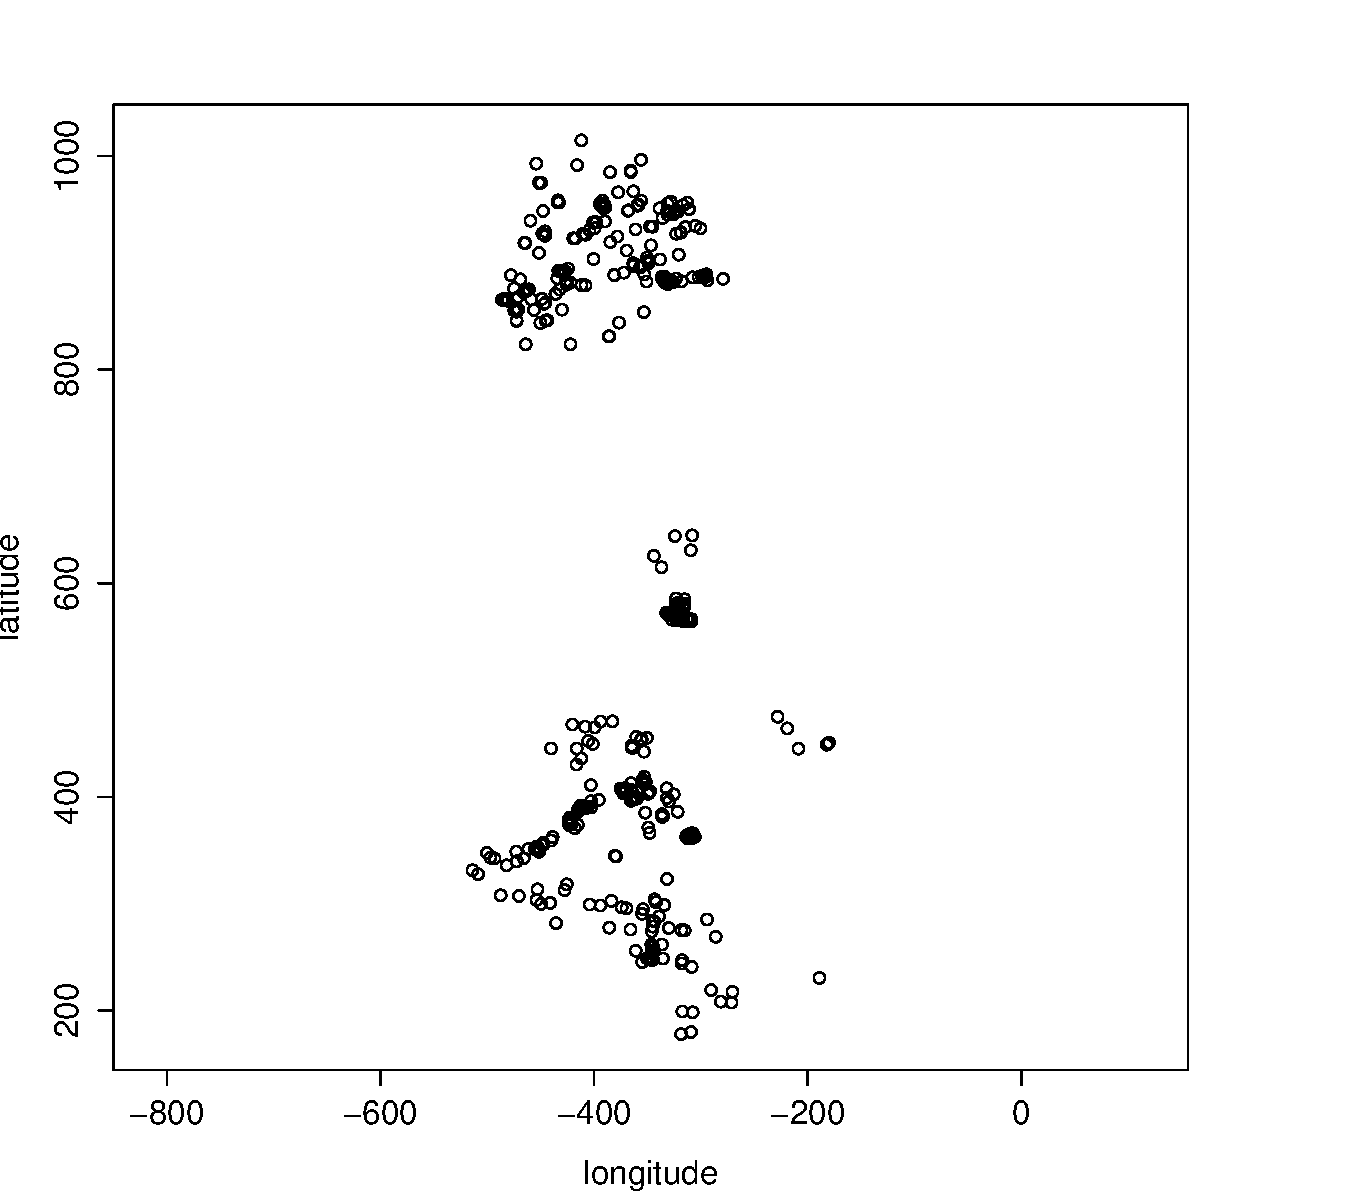
\includegraphics[width=12cm]{Downscaling-downscale30}
\end{figure}

\newpage
Now we have to convert these points in to a coarse-scale raster. The simplest method is to bound our raster by the limits of the location coordinates. Careful thought must also be put in to the grain size. It must be large enough that we are confident it is an accurate representation of presence-absence, but also small enough to allow upgraining to give at least three spatial scales worth of occupancy data for fitting the downscaling models. In the UK butterflies are generally sampled at a 10 km grid cell, so we'll set a grain size of 20 km width (400 km$^2$), which gives us a little more certainty in our atlas data but will still comfortably allow us to upgrain to give three scales (400, 1600, 6400 km$^2$).

\begin{Schunk}
\begin{Sinput}
## set grain size as 20 km
cell.width <- 20

# extract extent of coordinates
coords.extent <- extent(records.coords)

## create a blank raster to fit the coordinates (note the addition of half a 
## cell width on all sides)
gbif_raster <- raster(xmn = coords.extent@xmin - (cell.width / 2),
                      xmx = coords.extent@xmax + (cell.width / 2),
                      ymn = coords.extent@ymin - (cell.width / 2),
                      ymx = coords.extent@ymax + (cell.width / 2),
                      res = cell.width)
                      
## assign cells with presence records as 1
gbif_raster <- rasterize(records.coords, gbif_raster, field = 1)

## convert cells with NA (no records) to 0
gbif_raster[is.na(gbif_raster)] <- 0

plot(gbif_raster, legend = FALSE)
\end{Sinput}
\end{Schunk}

\begin{figure}[!ht]
\centering
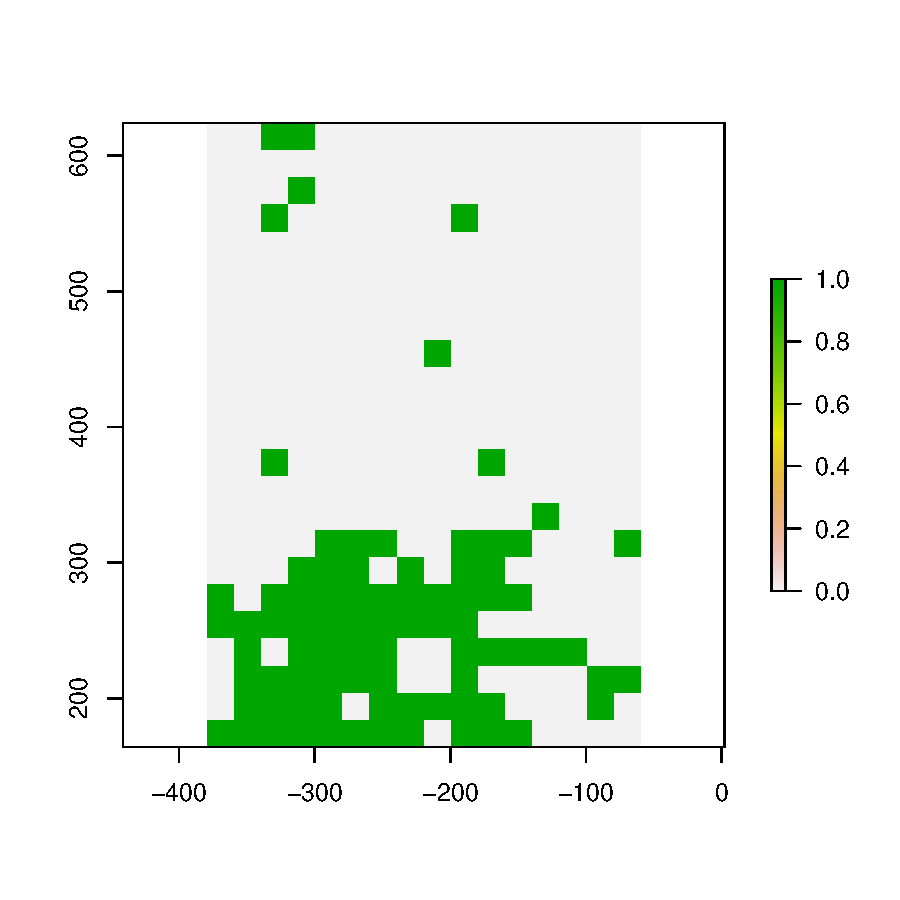
\includegraphics[width=8cm]{Downscaling-downscale32}
\end{figure}

As our area is rectangular we should not be too worried about setting our thresholds for upgraining, and so we can choose the “All\_Sampled” option to maintain all data.

\begin{Schunk}
\begin{Sinput}
occupancy <- upgrain(gbif_raster,
                     scales = 2,
                     method = "All_Sampled")
\end{Sinput}
\end{Schunk}

We can see there has not been much increase in extent after upgraining:

\begin{Schunk}
\begin{Sinput}
## The extent of the original atlas data
occupancy$occupancy.orig[1, 2]
\end{Sinput}
\begin{Soutput}
[1] 163200

\end{Soutput}
\begin{Sinput}
## The extent of the standardised atlas data
occupancy$extent.stand
\end{Sinput}
\begin{Soutput}
[1] 192000

\end{Soutput}
\end{Schunk}

\begin{figure}[!ht]
\centering
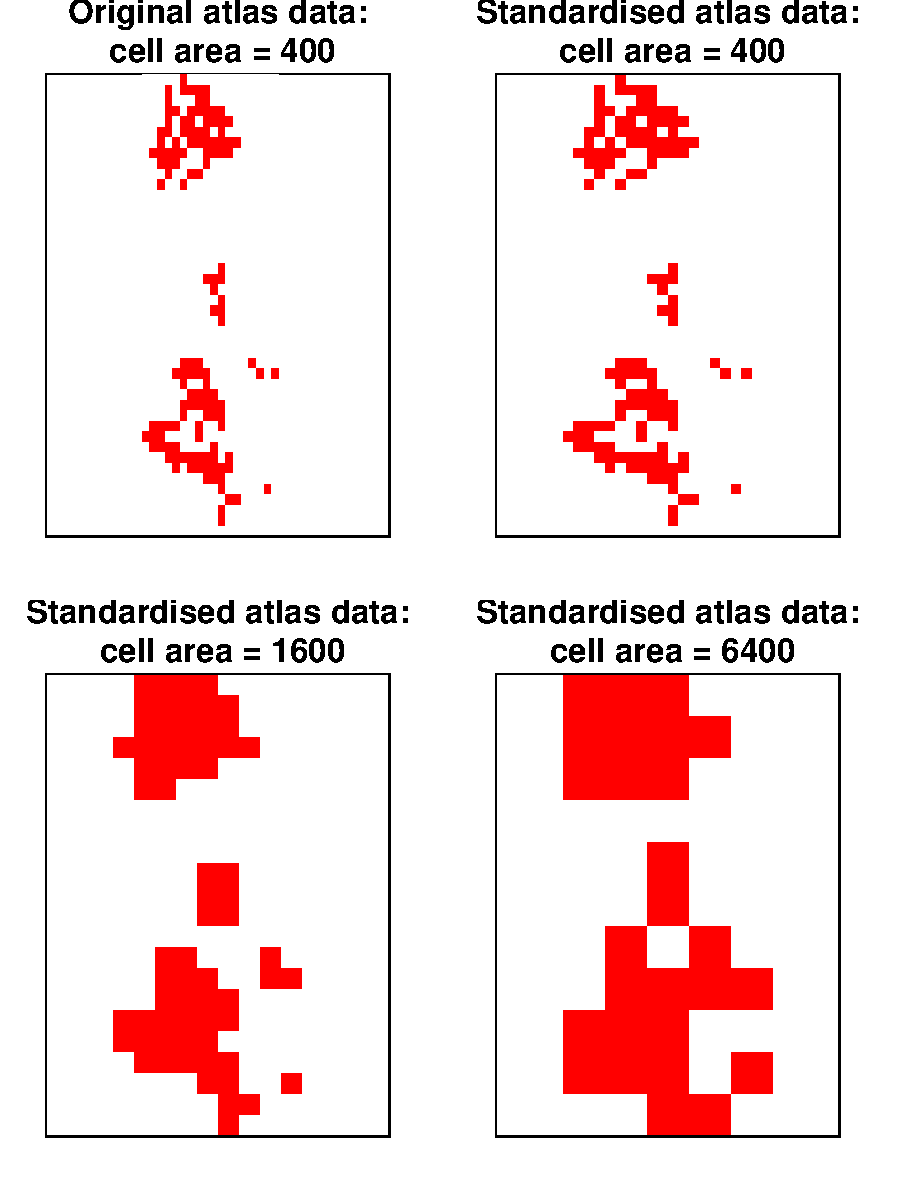
\includegraphics[width=9.5cm]{Downscaling-downscale33}
\end{figure}

\newpage
Now we can run our ensemble downscaling models:

\begin{Schunk}
\begin{Sinput}
ensemble <- ensemble.downscale(occupancy,
                               models = "all",
                               new.areas = c(1, 10, 100, 400, 1600, 6400),
                               tolerance_mod = 1e-3)
\end{Sinput}
\begin{Soutput}
Nachman model is running...  complete 
PL model is running...  complete 
Logis model is running...  complete 
Poisson model is running...  complete 
NB model is running...  complete 
GNB model is running...  complete 
INB model is running...  complete 
FNB model is running...  complete 
Thomas model is running...  complete 
Hui model is running...  complete

Warning message:
In predict.downscale(object = mod, new.areas = new.areas, extent = extent,  :
  Predicted results may be innaccurate: one or more 0's predicted.
\end{Soutput}
\end{Schunk}

\begin{figure}[!ht]
\centering
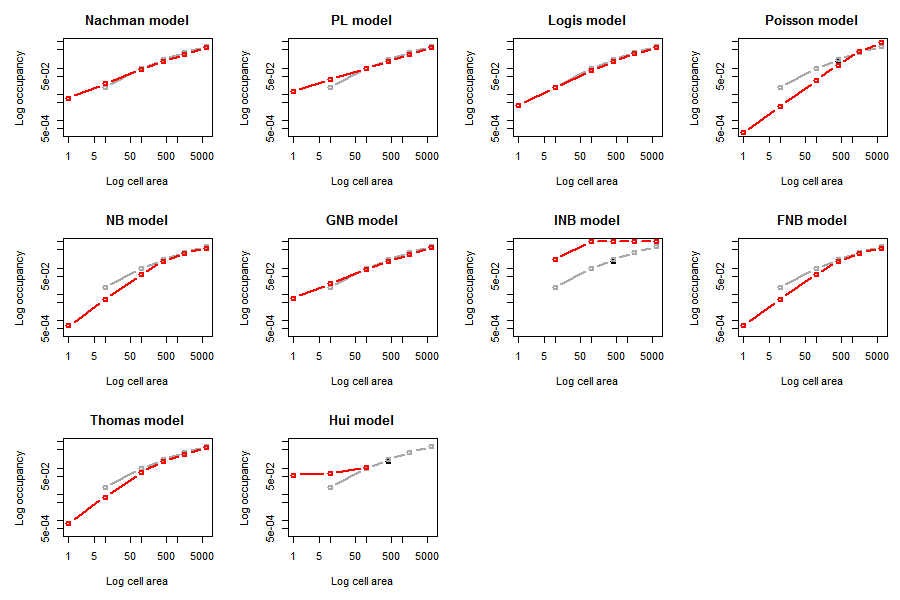
\includegraphics[width=\linewidth]{Downscaling-downscale34}
\end{figure}

\newpage
The INB model has not converged satisfactorily and thrown up a warning message (it has predicted a 0 at the finest grain size which we know to be impossible). This highlights the importance of visually inspecting the model fits. We can try tweaking it’s starting parameters to see if we can get a better fit using the \texttt{starting\_params} argument:

\begin{Schunk}
\begin{Sinput}
ensemble <- ensemble.downscale(occupancy,
                               models = "all",
                               new.areas = c(1, 10, 100, 400, 1600, 6400),
                               tolerance_mod = 1e-3,
                               starting_params = list(INB = list(C = 10, 
                                                                 r = 0.01, 
                                                                 b = 0.1)))
\end{Sinput}
\begin{Soutput}
Nachman model is running...  complete 
PL model is running...  complete 
Logis model is running...  complete 
Poisson model is running...  complete 
NB model is running...  complete 
GNB model is running...  complete 
INB model is running...  complete 
FNB model is running...  complete 
Thomas model is running...  complete 
Hui model is running...  complete 





\end{Soutput}

\begin{Sinput}
## And the predicted mean area of occupancies for each grain size
ensemble$AOO[, c("Cell.area", "Means")]
\end{Sinput}

\begin{Soutput}
  Cell.area       Means
1         1    617.8954
2        10   2966.7477
3       100  13958.6322
4       400  32781.6381
5      1600  68197.5079
6      6400 117253.2752
\end{Soutput}
\end{Schunk}

\begin{figure}[!ht]
\centering
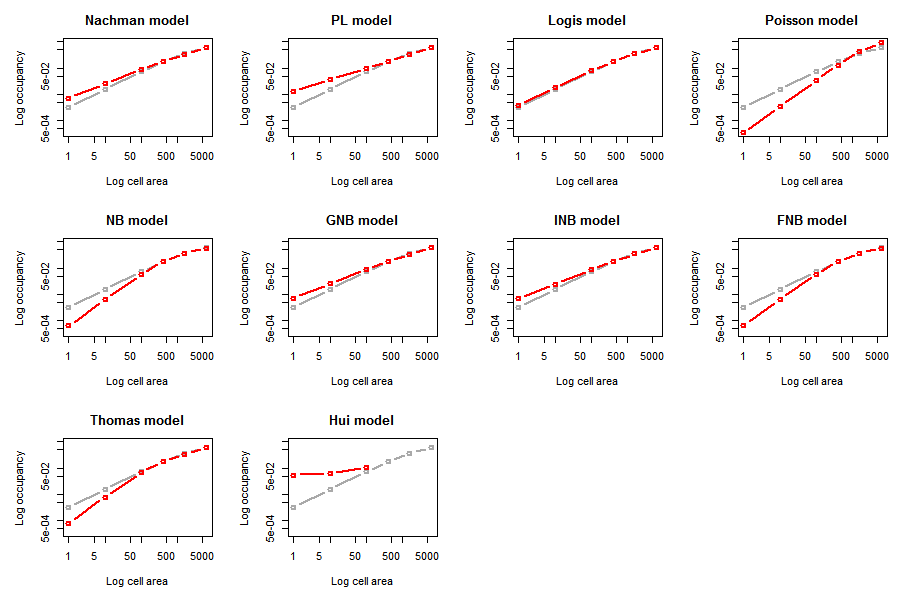
\includegraphics[width=\linewidth]{Downscaling-downscale36}
\end{figure}

So far we have simply drawn a rectangle around our points, but perhaps we have a better idea of the possible range limits of the species. In our case, it is probably sensible to set the extent as mainland UK. A shapefile of the UK has been provided which we can load in.

\begin{Schunk}
\begin{Sinput}
uk <- system.file("extdata", "UK.shp", package = "downscale")
uk <- shapefile(uk)

## reproject to be the same coordinate system as our GBIF data (in km)
uk <- spTransform(uk,
                  CRS("+proj=lcc +lat_1=49.8333339 +lat_2=51.16666733333333
                       +lat_0=90 +lon_0=4.367486666666666 +x_0=150000.01256 
                       +y_0=5400088.4378 +ellps=intl +units=km +no_defs"))

## plot our GBIF records on top of the UK polygon
plot(uk)
plot(records.coords, add = TRUE, col = "red)
\end{Sinput}
\end{Schunk}

\begin{figure}[!ht]
\centering
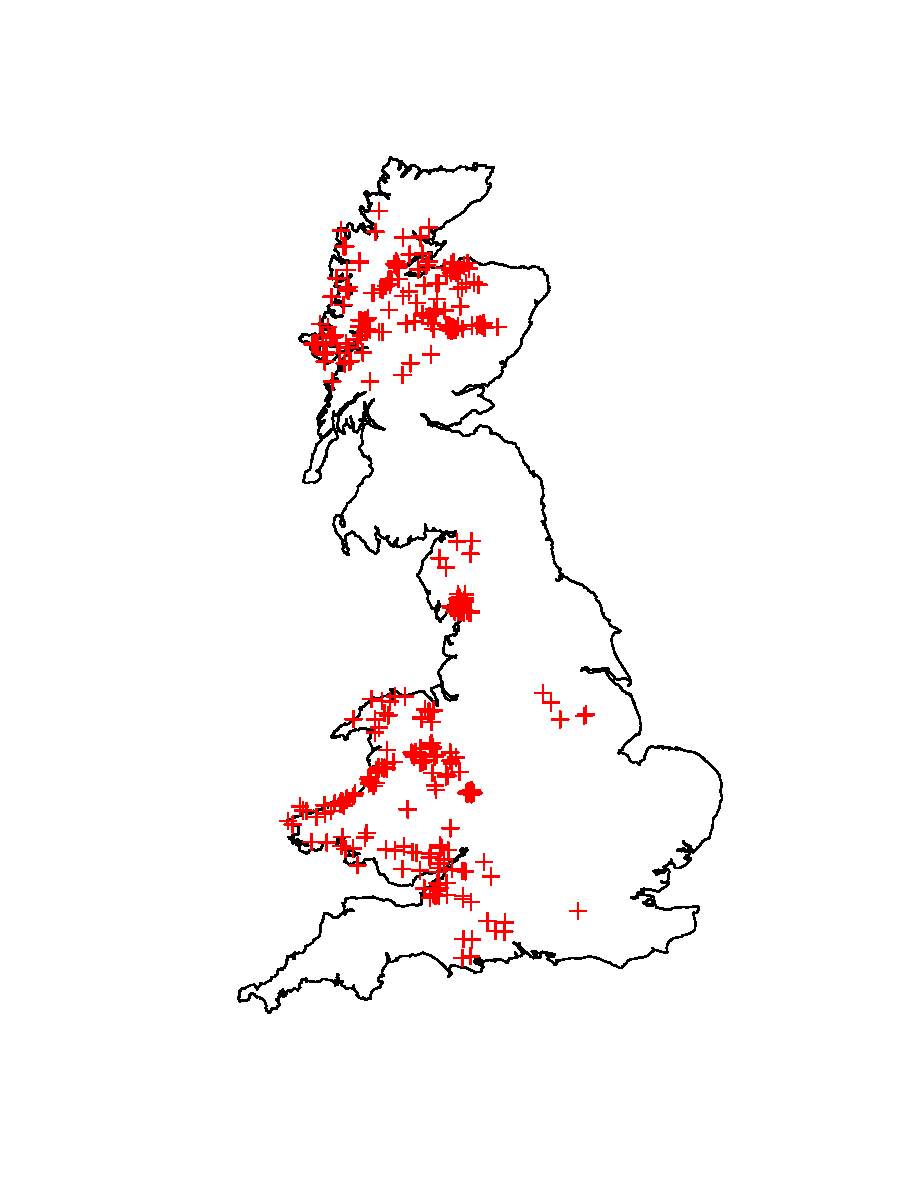
\includegraphics[width=10cm]{Downscaling-downscale38}
\end{figure}

\newpage
Now, we make our raster of presence-absence the same way as before, except this time we set the extent to be the same as that of the polygon. We then mask the raster file with the UK polygon so that any cells outside this polygon are assigned as NA (unsampled cells):

\begin{Schunk}
\begin{Sinput}
## create a blank raster with the same extent as the UK polygon
gbif_raster <- raster(ext = extent(uk),
                      res = cell.width)

## assign cells with presence records as 1
gbif_raster <- rasterize(records.coords, gbif_raster, field = 1)

## convert cells with NA (no records) to 0
gbif_raster[is.na(gbif_raster)] <- 0

## mask the raster to the UK polygon, so cells outside the polygon are NA
gbif_raster <- mask(gbif_raster, uk)

## plot the masked atlas raster and overlay with the UK polygon
plot(gbif_raster, legend = FALSE)
plot(uk, add = TRUE)
\end{Sinput}
\end{Schunk}

\begin{figure}[!ht]
\centering
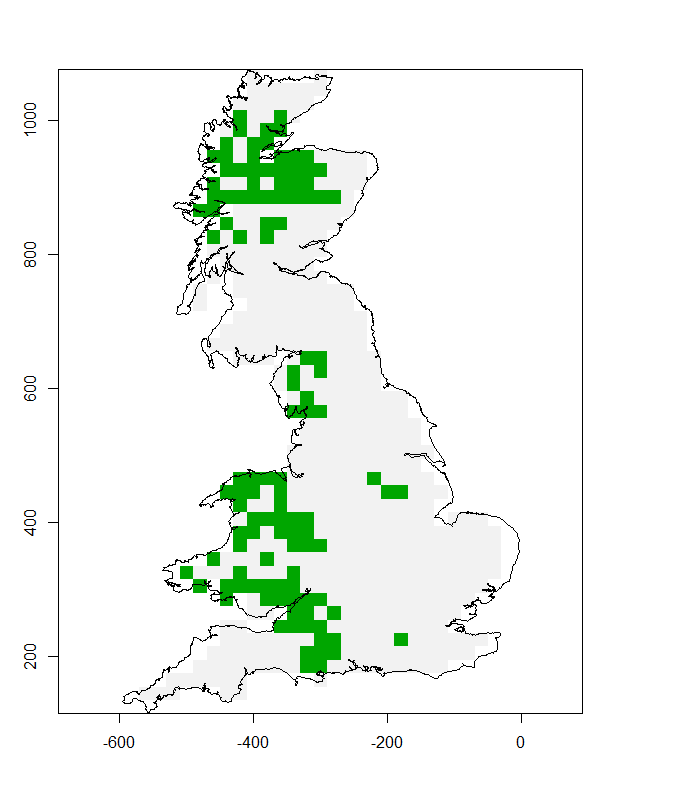
\includegraphics[width=10cm]{Downscaling-downscale40}
\end{figure}

\newpage
Now, we just upgrain and downscale as before:

\begin{Schunk}
\begin{Sinput}
occupancy <- upgrain(gbif_raster,
                     scales = 2,
                     method = "All_Sampled")
\end{Sinput}
\end{Schunk}

\begin{figure}[!ht]
\centering
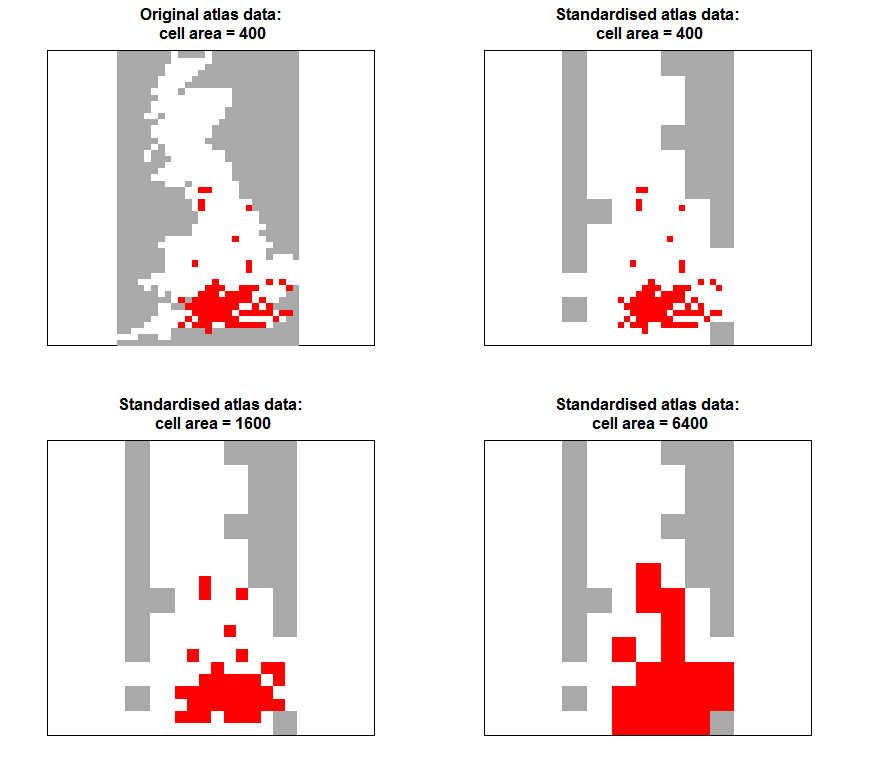
\includegraphics[width=9.5cm]{Downscaling-downscale41}
\end{figure}

\setkeys{Gin}{width=1\linewidth}
\begin{Schunk}
\begin{Sinput}
ensemble <- ensemble.downscale(occupancy,
                               models = "all",
                               new.areas = c(1, 10, 100, 400, 1600, 6400),
                               tolerance_mod = 1e-3,
                               starting_params = list(INB = list(C = 10,
                                                                 r = 0.01,
                                                                 b = 0.1)))
\end{Sinput}
\begin{Soutput}
Nachman model is running...  complete 
PL model is running...  complete 
Logis model is running...  complete 
Poisson model is running...  complete 
NB model is running...  complete 
GNB model is running...  complete 
INB model is running...  complete 
FNB model is running...  complete 
Thomas model is running...  complete 
Hui model is running...  complete 
\end{Soutput}

\begin{Sinput}
## And the predicted mean area of occupancies for each grain size
ensemble$AOO[, c("Cell.area", "Means")]
\end{Sinput}

\begin{Soutput}
  Cell.area       Means
1         1    665.2036
2        10   3353.7223
3        25   6408.7945
4       100  17003.7297
5       400  43131.0685
6      1600  98390.5784
7      6400 183332.8997
\end{Soutput}
\end{Schunk}

\begin{figure}[!ht]
\centering
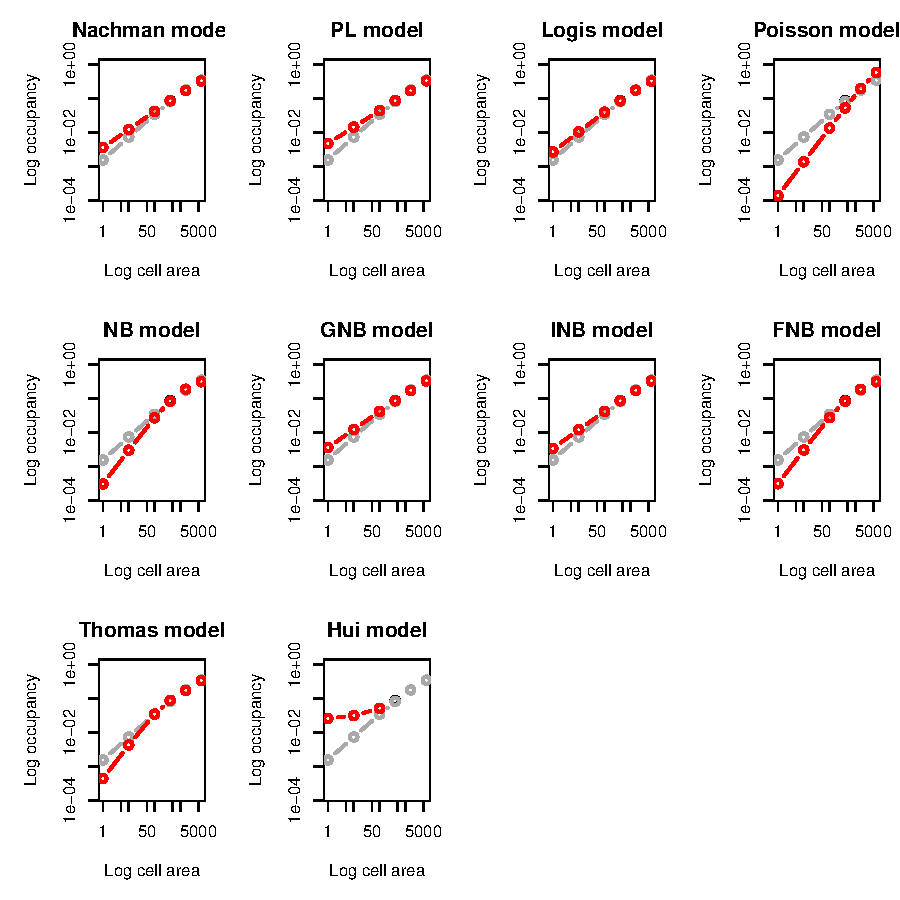
\includegraphics[width=\linewidth]{Downscaling-downscale42}
\end{figure}

If we want to compare predicted occupancy between the two methods we must compare the converted area of occupancies (AOO), not the proportion of occupancies as these are calculated from different extents. In this case the estimates for grain sizes of 1 km and 10 km from the bounded rectangle (AOO = 618 km$^2$ and 2967 km$^2$) are quite a bit larger than the estimates using the full mainland UK (AOO = 556 km$^2$ and 2635 km$^2$), most likely as a lot of cells in the atlas generated by the bounded rectangle would actually be sea. This highlights the care that is needed in selecting the bounding extent, the method and number of scales to upgrain, and the grain size we wish to predict occupancy for.

\section{Bibliography}

Azaele, S., S. J. Cornell, and W. E. Kunin. 2012. Downscaling species occupancy from coarse spatial scales. Ecological Applications 22:1004–14.

Barwell, L. J., S. Azaele, W. E. Kunin, and N. J. B. Isaac. 2014. Can coarse-grain patterns in insect atlas data predict local occupancy? Diversity and Distributions 20:895–907.

Hartley, S., and W. E. Kunin. 2003. Scale dependence of rarity, extincition risk, and conservation priority. Conservation Biology 17:1–12.

Hui, C., M. A. McGeoch, B. Reyers, P. C. le Roux, M. Greve, and S. L. Chown. 2009. Extrapolating population size from the occupancy-abundance relationship and the scaling pattern of occupancy. Ecological Applications 19:2038–2048.

Hui, C., M. A. McGeoch, and M. Warren. 2006. A spatially explicit approach to estimating species occupancy and spatial correlation. Journal of Animal Ecology 75:140–147.

IUCN. 2014. Guidelines for using the IUCN Red List categories and criteria.

Kunin, W. E. 1998. Extrapolating species abundance across spatial scales. Science 281:\\
1513–1515.

\end{document}
